\begin{savequote}[75mm]
Science isn't about WHY, it's about WHY NOT!
\qauthor{J.K. Simmons (Portal 2)}
\end{savequote}
\chapter{Machine Learning methods and analysis for strip Velo}
\label{chap:ml-velo}

%This chapter is dedicated to the research related to the Velo detector monitoring and the possibility of application of machine learning methods for these purposes. The scope of the work relates to the version of Velo used in LHC Runs 1 and 2. These studies have been conducted in different timespans. So for the section \ref{chap4:run12} the data used in analysis were collected between years 2010-2017 whilst the data pertaining to the methods described in \ref{chap4:dimred} and \ref{chap4:wtte} also included the year 2018. The structure this chapter keeps the chronological order of the conducted studies. The big picture and the main motivation of the presented work are to use the large data sets collected during the operation of the commissioned detector to prepare high quality monitoring algorithms for the upgraded one.

The particle beam present at the LHC, while being a source of particle colissions that can unveil mysteries of the universe, is also constantly damaging the detector.
The more particles is there flowing through the detector, the more the detector is damaged, the less the particles it will detect.
The role of the maintainers of the detector is to balance on the edge of destruction of the detector, and expansion of knowledge.
This carefull ballet motivates the work presented in this Chapter.
The studies presented here, are hoped to foster the balance, by providing quick insights into detector behaviour.

The first Section (\ref{chap4:run12}) of this Chapter provides analysis of the calibration parameters of the Velo detector in years 2010-2017. This analysis shows how the radiation damage influences the calibration, and puts the bias voltage correction to the ultimate test. 
Additionally, using probabilistic programming and the insight from the analysis, we present an intelligent method for finding anomalious calibrations (Sec. \ref{chap4:outlierness}). Which was succesfully implemented to the Velo monitoring.

The changes in the calibration may be elusive to a human operator, given a number of silicon strips (170 000).
The usual plots and visualisation tools might not suffice to reflect the overall picture, and so we present the study of the dimensionality reduction techniques (PCA and autoencoders) applied on the calibration data (Sec. \ref{chap4:dimred}). 

Next (Sec. \ref{chap4:wtte}), we answer he question: how does the calibration influence the signal? The answer led us to developing a tool that can help to a detector maintainer to decide about the timing of the calibration.
The calibration process requires a specific condition of the detector, and must be carefully scheduled.

In summary, these studies are meant to equip the detector maintainers with intelligent tools that will enhance the data taking, mainly in Run 3 at the LHCb, but also the detectors to which these methods might be transferable.


  % /////////////////////////////////////////////////////////////////////////
  %
  %
  %
  %
  %                             NEW SECTION
  %
  %
  %
  %
  %
  %



\section{Run 1 and 2 calibration analysis}
\label{chap4:run12}

Runs 1 and 2 of the LHC machine were the initial runs of the Large Hadron Collider. Run 1 started in 2011 and lasted to the end of 2012, and Run 2 lasted from 2015 to 2018\cite{Hoecker:2236645}.
Because of the global pandemic, the plans for the years 2019-2022 changed, and the LHC actually will start taking data in 2022 (Fig. \ref{plot:lhc_schedule}).
Although the detector operated nominally throughout the time of its working, the study of its behaviour was needed to ensure that the Velo team at LHCb had a complete picture of its condition. The Velo being one of the core detectors, capable of performing the stand alone tracking and vertexing, provided the vital input for the physics programme.

\begin{sidewaysfigure}
    \centering
    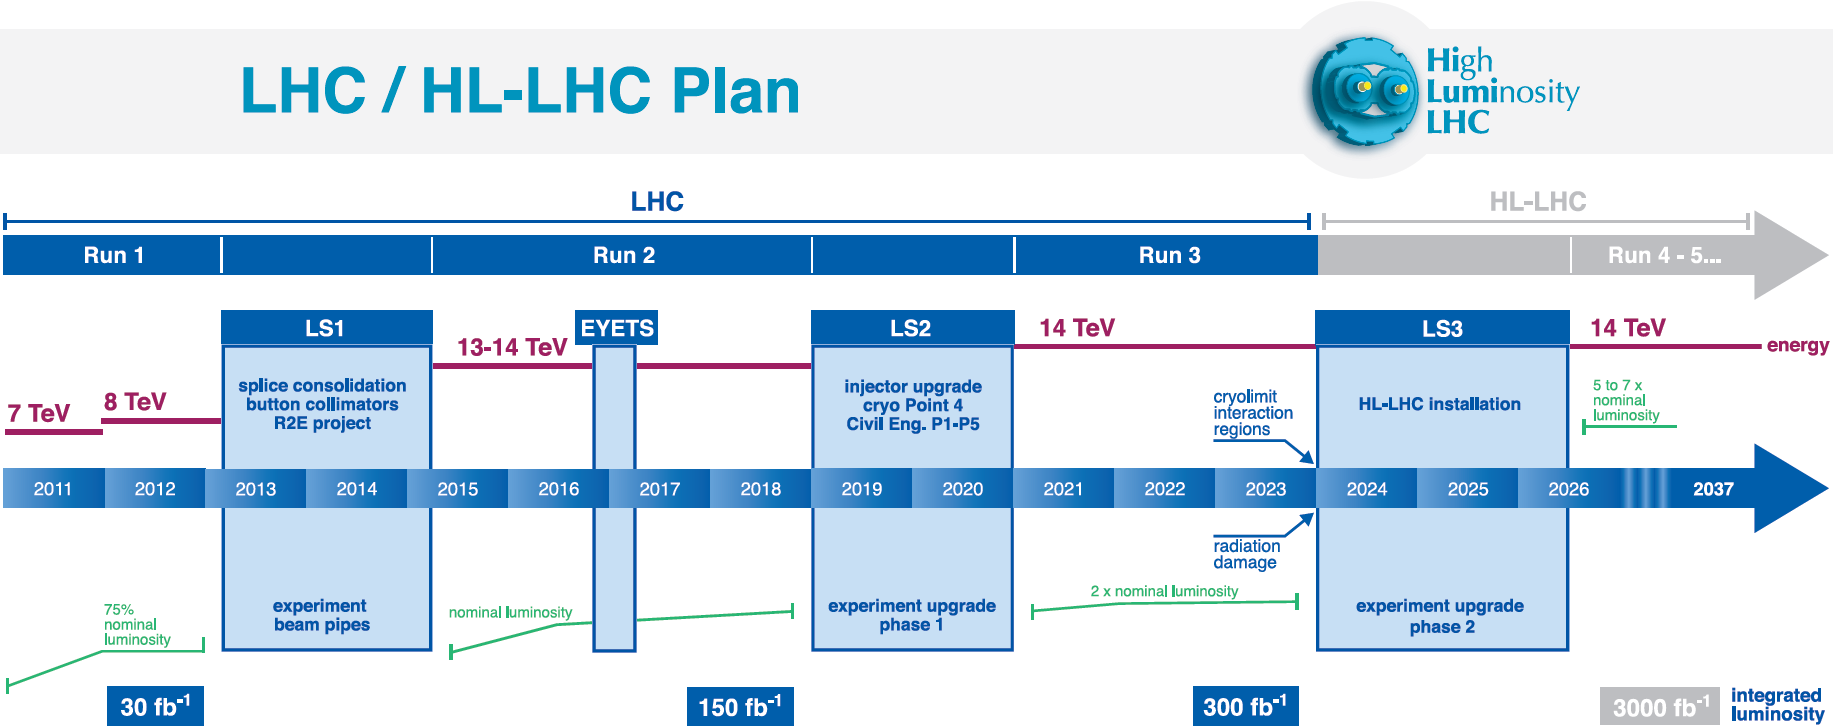
\includegraphics[width=0.9\linewidth]{figures/chapter4/lhc_schedule.png}
    \caption{The schedule of the runs from 2019. This schedule has already been changed for 2020 due to the global pandemic.}
    \label{plot:lhc_schedule}
\end{sidewaysfigure}

\subsection{The Data}

The data used in this Section comes from a timespan 2010-08-18 to 2017-06-21 and contains 30 Velo calibrations.
%It relates to the calibration data.

%The most significant for the Velo set of data are the following parameters:
Out of many different parameters the following ones were considered the most vital for the daily operation of the Velo detector:
\textbf{Pedestals} $P$, \textbf{Low Threshold} $L_t$ and \textbf{High Threshold} $H_t$.
As discussed in the Sn \ref{chap2:calibration}
Low Threshold and High Threshold only differ in scaling factor, so in further analysis, only high threshold and pedestal parameters will be used in this Section.


%This data is difficult the analysis because of the scope of its dimensionality. 
The dimensionality and complicated nature of the Velo calibration dataset pose a serious problem for their efficient analysis.
A single Velo sensor has 2048 readout channels, which constitutes the channel dimension. The sensors are of two types $R$ and $\phi$-type for each of the 42 modules, creating sensor-type and module number dimensions. Finally, each calibration is distinguished by the calibration date. This is summarised in Table \ref{tab:velo_dimentionality}.

\begin{table}[h]
\begin{center}
\begin{tabular}{ |c|c|c| }
\hline
Dimention name & Symbol & Size\\
\hline
Channel & $Ch$ & 2048\\
Sensor type & ${R, \phi}$ & 2 ($R$ or $\phi$) \\
Module number & $\#$ & 42 \\
Calibration date & $T$ & 30\\
\hline
\end{tabular}
\caption{\label{tab:velo_dimentionality}Table of dimentionality of the calibration dataset.}
\end{center}
\end{table}

As mentioned above, the dimensionality in this dataset is challenging to navigate and most certainly needs a visualisation tool that aggregates a part of it.
The most helpful graphical object for handling this kind of data is 2D histogram, where the channel number is defined on X-axis (horizontal), and a given parameter ($H_{t}$ or $P_{t}$) value on the Y-axis (vertical), Example: Fig. \ref{plot:part1-r-phi-pedestals}.
The colour of the histogram is the number of occurrences of a given parameter value in a given bin.
When there is no occurrence of pairs of values, the colour is set to white for easier differentiation.
In this Chapter, the colour scale is different for each plot unless mentioned otherwise.
I do not provide the exact colour scale in most plots, but it follows the intuitive rule of warmer colours meaning more occurrences.
This kind of figure has proved to be very useful since it can aggregate multiple dimensions of the data.

For ease of understanding, I introduce the following notation of the dataset slice: 

$ParameterType(Ch, S, \#, D)$, 

where $ParameterType$ stands for the type of the parameter like $P$ or $H_t$ and the other symbols are explained in the Table \ref{tab:velo_dimentionality}.
A single symbol without values marks the use of a full range of data on that dimension.
Exemplary notation: $P(Ch100-Ch500, R, \#11, D)$ is a slice of R-type sensor channels from 100 to 500 in module $\#11$ in all of the calibrations. As one can see, even the slicing procedure is quite challenging and needs to take into account many aspects of the whole calibration dataset collected for Velo during its operation.

\subsection{Pedestals}

Pedestals represent the absolute electronics offsets measured in each detector readout channel. Their variations have proven to influence the data taking significantly (see Sec. \ref{chap4:wtte}). A special procedure, called noise data taking, was designed and put in place for Run 1 and Run 2 in order to evaluate the pedestals for each individual channel of the Velo detector.
Basic exploratory analysis of this parameter starts with an overall look at all pedestal values in the calibration dataset (see Fig. \ref{plot:part1-r-phi-pedestals}).
The pedestals oscillates around 520 ADC, with visible artefacts at channels 1400-1520 in $R$-type type sensor and near channel 1750 in both sensor types.
The first artefact (ranges 1400-1520) comes solely from the sensor \#85
% (@TODO recast senor number ????)
, visible in the Fig. \ref{plot:par1-pedestal-sensors}. This is believed to be a sensor malfunction (a visual inspection identified surface cracks). 
The other artefact near channel 1750 is believed to be coming from a design feature, identified as coupling to the digital clock line. 
This is not a significant problem for the overall data quality, since the effects can be precisely evaluated and seem to be fixed in time.


\begin{figure}
    \centering

    \begin{subfigure}[b]{\textwidth}
    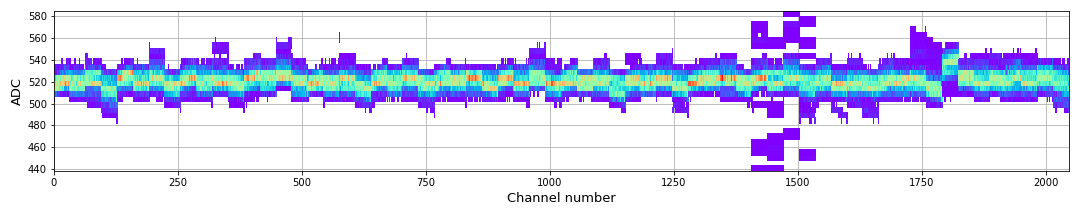
\includegraphics[width=\linewidth]{figures/chapter4/calib_analysis/Part1-phi-pedestals.png}
    \caption{All phi pedestals.}
   \label{plot:ped_r}
  \end{subfigure}

  \begin{subfigure}[b]{\textwidth}
    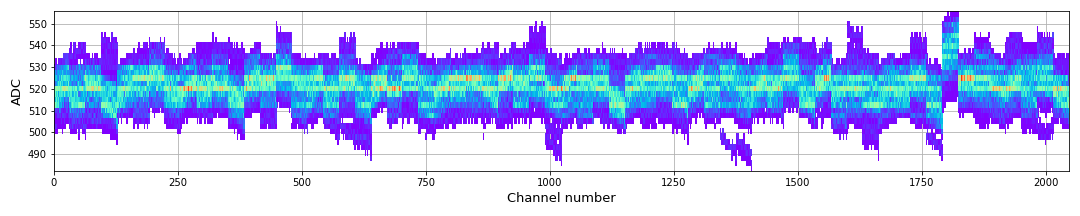
\includegraphics[width=\linewidth]{figures/chapter4/calib_analysis/Part1-r-pedestals.png}
    \caption{All $R$-type pedestals.}
   \label{plot:ped_phi}
  \end{subfigure}
      % \caption[All calond]{All of the calibrations, with reduced dimentionality using autoencoder and PCA.}
    \caption{Histogram of the all of the pedestal values across all of the calibrations The histogram above is $P_{Ch, R, \#, T}$ and the below $P(Ch, \phi, \#, T)$).}
    \label{plot:part1-r-phi-pedestals}

  \end{figure}

% \begin{figure}
%     \centering
%     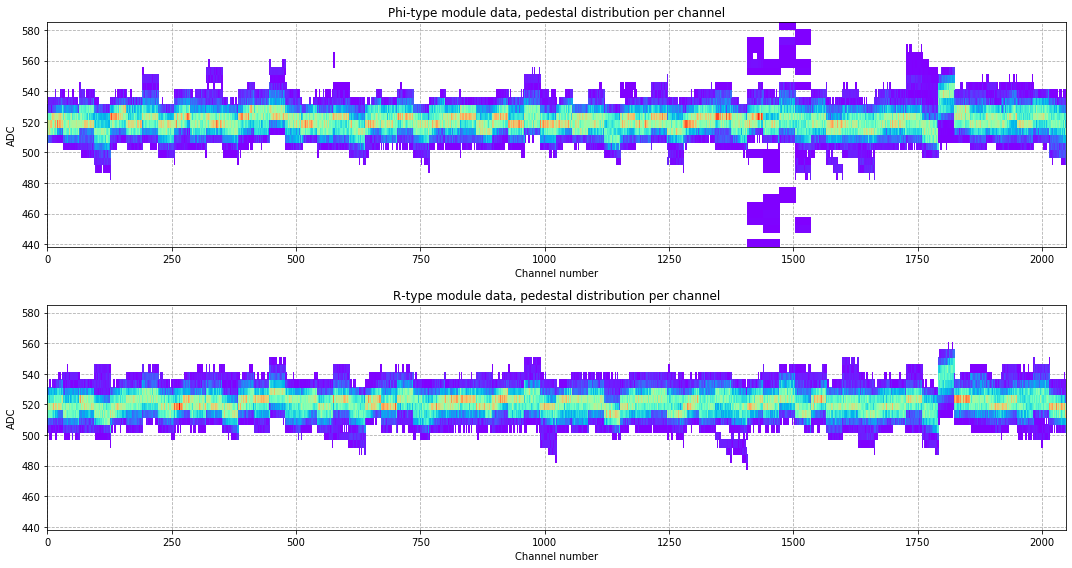
\includegraphics[width=0.7\linewidth]{figures/chapter4/calib_analysis/Part1-r-phi-pedestals.png}
%     \caption{Histogram of the all of the pedestal values, across all of the calibrations The histogram above is $P_{Ch, R, \#, T}$ and the below $P_{Ch, \phi, \#, T}$).}
%     \label{plot:part1-r-phi-pedestals}
% /\end{figure}

\begin{figure}
    \centering
    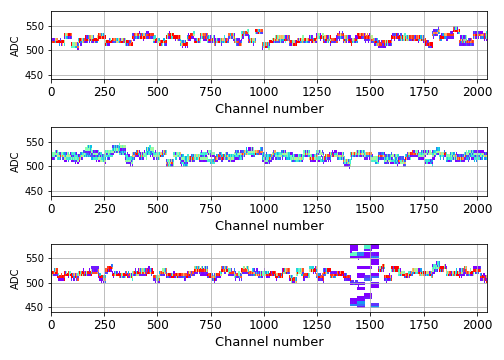
\includegraphics[width=0.7\linewidth]{figures/chapter4/calib_analysis/Part1-outliers-pedestals-cases.png}
    \caption{Pedestal plot for sensors (from the top) $P(Ch, R, \#64, T)$ $P(Ch, R, \#35, T)$ $P(Ch, R, \#85, T)$. $\#64$ and \#35 represent a typical pedestal values, while in \#85 there is a malfunction visible close to channel 1500.}
    %@TODO recast the sensors to their modules, and check the sensor type
    % - im leaving this comment since i don't remember what this was about exactly
    % - but the sensor type matches the description
    \label{plot:par1-pedestal-sensors}
\end{figure}

The intense mixed radiation field, consisting of fast hadrons, gradually damaged the sensors during their operation, resulting in the need to adjust the bias voltage.
%The pedestal parameter is actually a way of fine-tuning the signal levels.
%If the value of the pedestals would exhibit a trend, this could mean that the bias voltage adjustment is not sufficient or it doesn't give the desired result.
Proper estimation and correction for the pedestal value turned to be the critical part of the calibration procedure for Velo. The nature of this quantity is complicated and reflects the overall properties of the whole electronics readout chain. In principle it should not change significantly over time under stable conditions of the hardware. Any strong variations could be interpreted as serious problems with the detector.
Thus, a study of the pedestal trend is an essential aspect of this analysis.
The trend was calculated by fitting a line $y=ax+b$ to the pedestal values using the time of the calibration as an independent variable.
The value of the linear coefficient $a$, which is responsible for the trend, is calculated individually for each of the detector channels.
The distribution of this coefficient is presented in the Fig. \ref{plot:part1-pedestal-trend}.
The mean value of the coefficient is $9.63e^{-5}$ which is so close to zero that it can be assumed that there is no overall trend, which proves that the detector did not suffer from any systematic effects, related to its hardware component, during the Run 1 and Run 2 data taking periods.

\begin{figure}
    \centering
    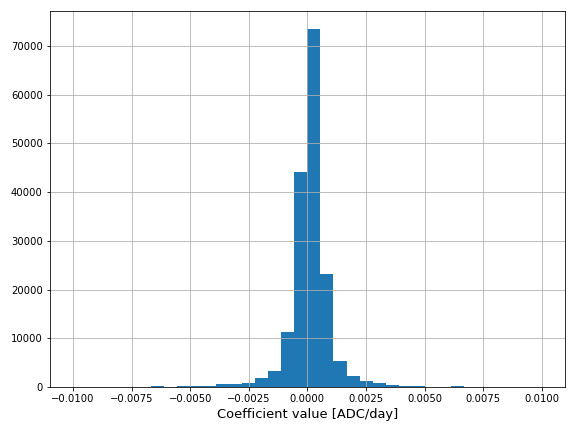
\includegraphics[width=0.7\linewidth]{figures/chapter4/calib_analysis/Part1-pedestal-trend.png}
    \caption{Histogram of linear coefficients of the pedestal trend per channel. Some of the outlying coefficient values have been trimmed and are outside the scope of this plot.}
    \label{plot:part1-pedestal-trend}
\end{figure}

\subsection{Clusterisation Thresholds}

The high threshold parameter, $H_{t}$, is the one actually responsible for the sensitivity the hit detection. It is one of the many steps of filtering the signal coming from Velo. Further, the hit information is crucial for the tracking algorithms that aggregate the collection of hits into a track and fit its trajectory (see Sec. \ref{chap2:calibration}).
Again, we start first at the simple exploratory analysis of the whole dataset. At the first glance, the 2D histograms presented in Fig. \ref{plot:part2-threshold-all} are cluttered by outlying values.
The most visible ones are near value 127 across all channels.
This is an expected sight, as value 127 is the maximal possible value.
Setting the value of the threshold in the channel to 127 means that only the signal that exceeds this threshold is accepted. Which, in reality, means that no signal will come through the channel as it would have to reach values greater than the dynamic range of the ADC value after the pedestal subtraction \footnote{The dynamic range of the Velo readout chain after signal digitisation and before pedestal subtraction is 10 bits without sign. Pedestal subtraction aims at equalisation of the properties of the readout channels across the detector. After the pedestal correction the dynamic range corresponds to 8 bits with sign, so effectively, we can observe signals in the range of -128 to 127 ADC counts.}. This, forces the data coming from such channels to be discarded.
This is a masking value, evolution of the distribution of those masks are discussed in detail in the next Section (\ref{chap4:masks}).
The other visible artefact are spikes within channel range fron 1000 to 1250.
This comes from faulty  sensor  \#67  and  dates  ’2016-11-07’  and  ’2016-11-11’,  where  the  threshold  values  reached non-physical value of 400  ADC. This is likely an error that could accidentally get into the dataset, and yet there is no explanation for those values (most likely an electrical disturbance influenced severely the global offset level).
Moving on, we will treat those values as outliers and remove from the analysis.

\begin{figure}
    \centering
    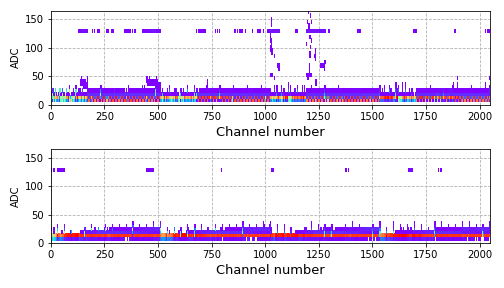
\includegraphics[width=0.7\linewidth]{figures/chapter4/calib_analysis/P2-threshold-all-r-phi.png}
    \caption{High threshold distribution of all of calibrations, across all sensors. $H_t(Ch,\phi,\#, D)$ is above, and $H_t(Ch,R,\#, D)$ is the plot below.}
    \label{plot:part2-threshold-all}
\end{figure}


The Fig. \ref{plot:P2-threshold-all-zoom} depicts $H_t(Ch, R, \#, D)$ and $H_t(Ch, \phi, \#, D)$ in range of values from 0 to 30.
One of the immediately visible features are the sparse spikes regularly distributed across the sensors.
Those spikes represent, so called, header cross-talk effect (Sec. \ref{chap2:headercrosstalk}), that affects specific channels during the analogue transmission of the data from the detector to the trigger processing farm.
In some cases, it might be helpful to exclude the channels that contain the header cross-talk effect.
The $Ch*$ denotes all of the channels without the header cross-talk effect.
The reader can examine the difference of the histogram with and without header cross-talk in the Fig. \ref{plot:P2-threshold-all-zoom} and \ref{plot:P2-threshold-all-zoom-nohc}.


\begin{figure}
    \centering
    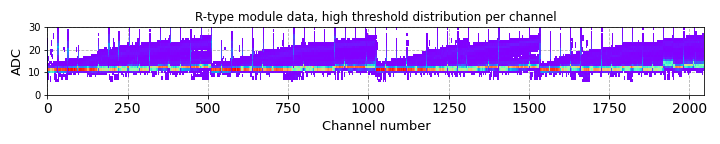
\includegraphics[width=\linewidth]{figures/chapter4/calib_analysis/P2-threshold-all-zoom.png}
    \caption{High threshold distribution with header cross-talk $H_t(Ch, R, \#, D)$.}
    \label{plot:P2-threshold-all-zoom}
\end{figure}

\begin{figure}
    \centering
    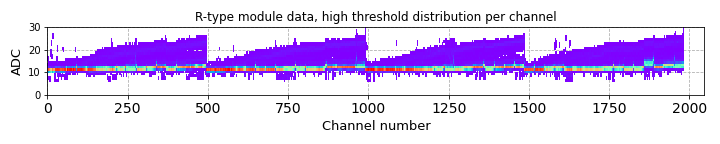
\includegraphics[width=\linewidth]{figures/chapter4/calib_analysis/P2-threshold-all-zoom-nohc.png}
    \caption{High threshold distribution without header cross-talk $H_t(Ch*, R, \#, D)$}
    \label{plot:P2-threshold-all-zoom-nohc}
\end{figure}


Another insight coming from the 2D histogram presented in Fig. \ref{plot:P2-threshold-all-zoom-nohc} is that low-intensity regularities repeat roughly every 512 channels. The periodicity of those regularities comes from the sensors' physical design and the specific topology of the strip implants.
More precisely, they are related to imperfect calibrations coming from two dates:  '2012-07-30', '2012-08-01'.
Those two dates are imperfect due to the improper response of the high voltage system that failed to provide bias voltage to the sensors on those dates. In consequence a very large noise was observed. The particular shape of the noise distributions for $R-$ and $\phi$-type sensors reflect the physical dimensions of the strips. For the former strip length increases gradually, in each of the sensor's four sectors, as a function of radius. For the latter strip length is constant for inner and outer sectors (with shorter strips in the inner region).
These imperfect calibrations influenced the sensitivity of the detector and impacted severly the Velo data quality. 
Additionally, for the purpose of outliers analysis, two calibration dates also are being recognised as imperfect 2012-08-02 and 2011-03-07.
The overall four imperfect calibrations can be seen in Fig. \ref{plot:all-bad-phi} and Fig. \ref{plot:all-bad-phi}.
Those occurrences of mis-calibrations were a direct motivation for detecting anomalies in the calibration in Section\ref{chap4:outlierness}. Lack of such automatic procedures led to data loss due to very low hit reconstruction efficiency of the Velo.

\begin{figure}
    \begin{subfigure}[b]{\textwidth}
    \centering
    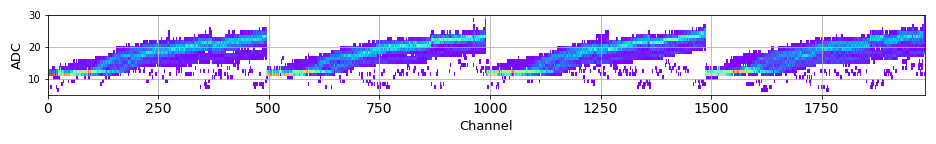
\includegraphics[width=0.9\linewidth]{figures/chapter4/calib_analysis/P2-all-bad-cals-R-0.png}
    \caption{$H_t(Ch*, R, \#, 2012-08-01), X=10$}
    \label{plot:all-bad-r-0}
  \end{subfigure}


    \begin{subfigure}[b]{\textwidth}
    \centering
    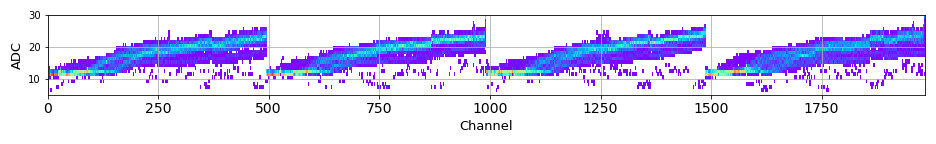
\includegraphics[width=0.9\linewidth]{figures/chapter4/calib_analysis/P2-all-bad-cals-R-1.png}
    \caption{$H_t(Ch*, R, \#, 2012-07-30), X=10$}
    \label{plot:all-bad-r-1}
  \end{subfigure}


    \begin{subfigure}[b]{\textwidth}
    \centering
    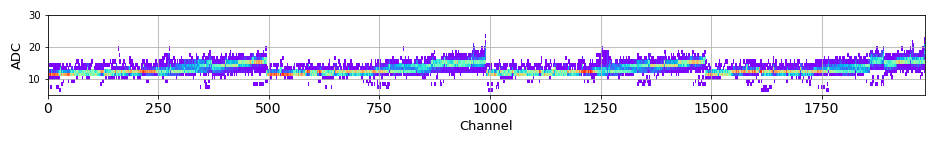
\includegraphics[width=0.9\linewidth]{figures/chapter4/calib_analysis/P2-all-bad-cals-R-2.png}
    \caption{$H_t(Ch*, R, \#, 2012-08-02), X=3$}
    \label{plot:all-bad-r-2}
  \end{subfigure}


    \begin{subfigure}[b]{\textwidth}
    \centering
    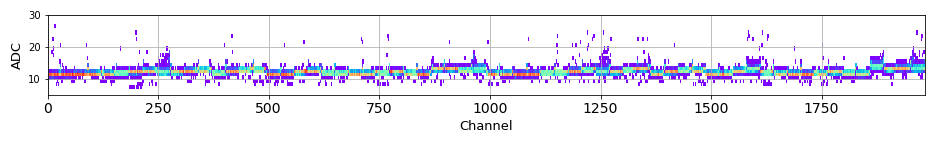
\includegraphics[width=0.9\linewidth]{figures/chapter4/calib_analysis/P2-all-bad-cals-R-3.png}
    \caption{$H_t(Ch*, R, \#, 2011-03-07), X=1$}
    \label{plot:all-bad-r-3}
  \end{subfigure}
    \caption{Histograms of imperfect calibrations in $R$-type sensors with their outlierness value $X$.}
\end{figure}

\begin{figure}

    \begin{subfigure}[b]{\textwidth}
    \centering
    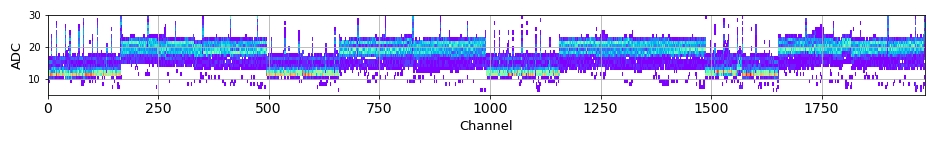
\includegraphics[width=0.9\linewidth]{figures/chapter4/calib_analysis/P2-all-bad-cals-phi-0.png}
    \caption{$H_t(Ch*, \phi, \#, 2012-08-01), X=10$}
    \label{plot:all-bad-phi-0}
  \end{subfigure}


    \begin{subfigure}[b]{\textwidth}
    \centering
    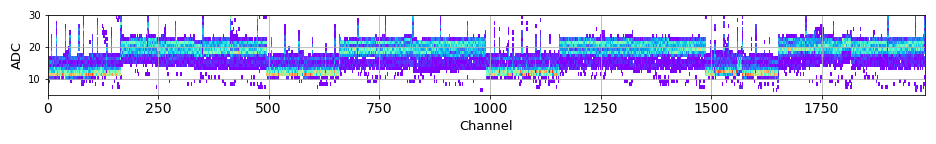
\includegraphics[width=0.9\linewidth]{figures/chapter4/calib_analysis/P2-all-bad-cals-phi-1.png}
    \caption{$H_t(Ch*, \phi, \#, 2012-07-30), X=10$}
    \label{plot:all-bad-phi-1}
  \end{subfigure}


    \begin{subfigure}[b]{\textwidth}
    \centering
    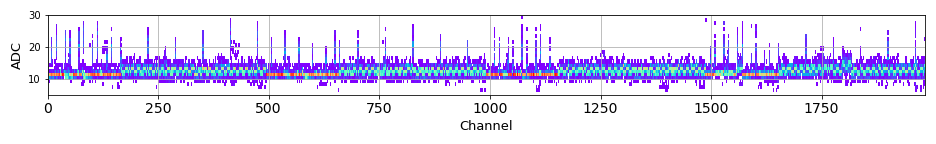
\includegraphics[width=0.9\linewidth]{figures/chapter4/calib_analysis/P2-all-bad-cals-phi-2.png}
    \caption{$H_t(Ch*, \phi, \#, 2012-08-02), X=3$}
    \label{plot:all-bad-phi-2}
  \end{subfigure}


    \begin{subfigure}[b]{\textwidth}
    \centering
    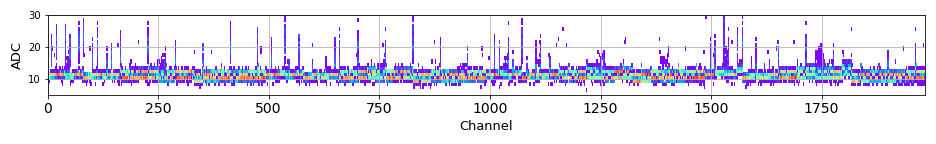
\includegraphics[width=0.9\linewidth]{figures/chapter4/calib_analysis/P2-all-bad-cals-phi-3.png}
    \caption{$H_t(Ch*, \phi, \#, 2011-03-07), X=1$}
    \label{plot:all-bad-phi-3}
  \end{subfigure}
    \caption{Histograms of imperfect calibrations in \phi sensors with their outlierness value $X$.}
    \label{plot:all-bad-phi}
\end{figure}


\begin{figure}
    \centering
    
    \begin{subfigure}[b]{\textwidth}
    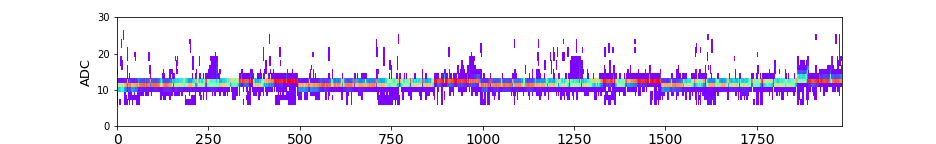
\includegraphics[width=\linewidth]{figures/chapter4/calib_analysis/P2-only-good-R.png}
    \caption{$H_t(Ch, \Phi, \#, 2012-08-02), X=0$}
   \label{plot:only_good_r}
  \end{subfigure}
  
  \begin{subfigure}[b]{\textwidth}
    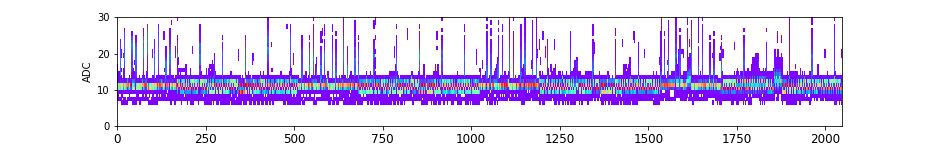
\includegraphics[width=\linewidth]{figures/chapter4/calib_analysis/P2-only-good-phi.png}
    \caption{$H_t(Ch, R, \#, 2012-08-02), X=0$}
   \label{plot:only_good_phi}
  \end{subfigure}
      \caption[All calond]{All of the calibrations, with reduced dimensionality using autoencoder and PCA.}
    \label{plot:only_good_all}
  
  \end{figure}

\subsection{Analysis of the outliers}
\label{chap4:masks}
As mentioned previously, the $H_t=127$ ADC means that the channel is masked.
Setting the threshold so high means that no hit will be registered in a given channel.
The masks were given to the channels that exhibited exceptional noise levels, were associated with broken or cold bonds, were connected to problematic readout chips or were close to sensor surface damage.
Their occurrences are depicted in Figs \ref{plot:p3-mask-time} and \ref{plot:p3-mask-time2}.
In  \ref{plot:p3-mask-time} the channels from all calibrations are plotted as a number of blocked channels per sensor in the time domain.
The important insight is that some sensors are more prone to masking than others and that the amount of masked channels changes.
In some cases, the masked channels can go away and return to the sensor.
The figure \ref{plot:p3-mask-time2}depicts a number of masked channels in the time domain with a sensor split.
It is clearly visible that the total number of masked channels grows with time.
This is expected as with time the negative radiation effects accumulate (see Sec. \ref{chap2:lumivolt}).

\begin{figure}
    \centering
    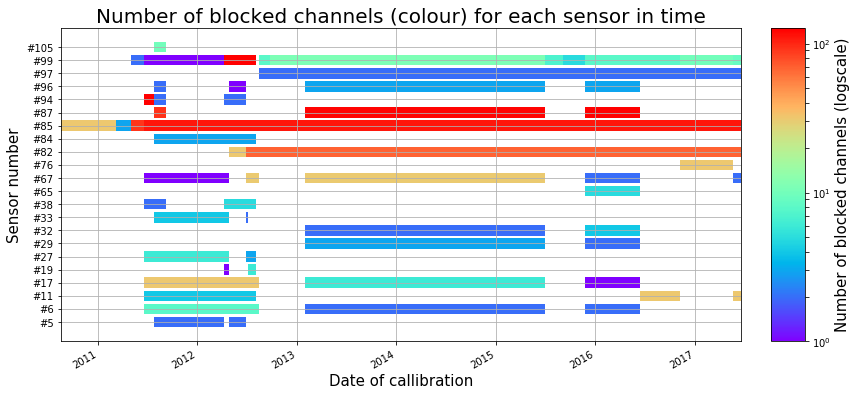
\includegraphics[width=0.95\linewidth]{figures/chapter4/calib_analysis/P3-mask-time.png}
    \caption{Distribution of blocked (masked) channels per sensor in time.}
    \label{plot:p3-mask-time}
\end{figure}

\begin{figure}
    \centering
    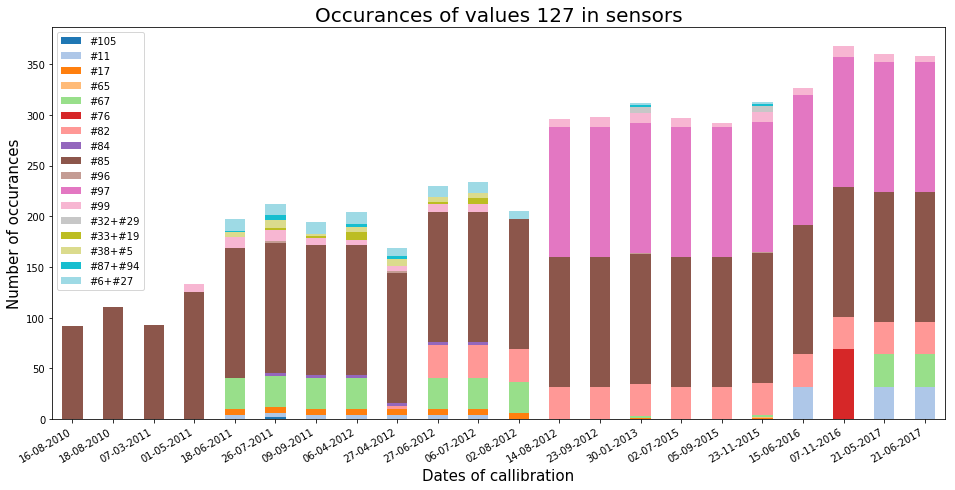
\includegraphics[width=0.95\linewidth]{figures/chapter4/calib_analysis/P3-mask-time2.png}
    \caption{The total number of occurrences of masked channels versus time.}
    \label{plot:p3-mask-time2}
\end{figure}

Apart from the masked values, the usual and outlying calibration, there is still a part of the data which doesn't fit any of those categories.
This part of data can be characterised as the $H_{t} > 50 ADC \land H_{t} \neq 127 ADC$.
Fig \ref{plot:p3-other-outliers} depicts those other outliers. The number of occurrences of these outliers changes from calibration to calibration, but overall is limited to three sensors: \#85 \#67 and \#94 (all $\phi$-type sensors). These anomalies have never been clearly characterised. The visual inspection did not indicate any surface damage on sensors, so that would point to instabilities in the electronics readout chain. Nevertheless, these bad channels were accounted for and did not affect the data quality.


\begin{figure}
    \centering
    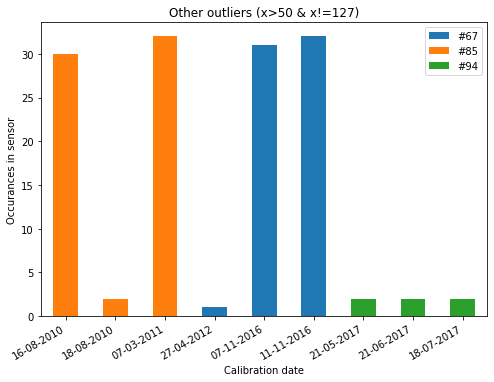
\includegraphics[width=0.7\linewidth]{figures/chapter4/calib_analysis/P3-other-outliers.png}
    \caption{Anomalous values other than masked channels.}
    \label{plot:p3-other-outliers}
  \end{figure}


  % /////////////////////////////////////////////////////////////////////////
  %
  %
  %
  %
  %                             NEW SECTION
  %
  %
  %
  %
  %
  %



\section{Intelligent analysis of the threshold data with probabilistic programming}
\label{chap4:outlierness}
The threshold evaluation procedure in the Velo directly influences the overall data taking quality in LHCb.
If the thresholds are too high, then there is a missing signal that decreases the precision of the track reconstruction and, in turn, decreases the trigger efficiency.
If the thresholds are too low, then the channel contributes to the noise and also may harm the quality of the data and stress the trigger system with a large number of fake hits.
Calibration process also requires time without beam, which is beyond the control of the LHCb and is the LHC collaboration responsibility.
To facilitate the correct calibration process, an additional check is advised.
The next Section presents the method for detecting anomalies in the calibration process.

\subsection{Dataset creation}
The exploratory analysis of the calibration data presented in the previous Section yielded a helpful insights into the properties of the high threshold, $H_t$, parameters.
Since high thresholds are evaluated using noise measured for each individual channel for $R$- and $\Phi$-type sensors we expect it to be within a well defined interval that should not depend on time \footnote{Properly configured detector should yield a noise that is approximately independent on time, however, there may be non trivial dependence on the radiation damage induced by fast hadrons.}.
It is assumed further that the distribution of the high thresholds should approximately follow a Gaussian distribution for properly configured detector. One should note, that the electronics noise has a number of components one of which is proportional to the strip capacitance, that in turn, is proportional to the strip length. For properly biased silicon sensors this component does not contribute significantly to the total noise, thus, we can assume the noise for $R$-type sensors stay constant within one ADC count. The same behaviour is measured for $\Phi$-type ones. Complete opposite behaviour is observed for the improperly configured sensors, i.e., the noise component proportional to the strip capacitance completely dominates the total noise value measured on each strip. This effect led to inventing an auxiliary variable, called ``outlierness'', that can quantify the departure of the noise distribution from the regular operation conditions.
%The analysis of the improper calibrations shows that the distribution of $H_t$ is also dependent on the channel (e.g. the regularity repeating every 500 channels).

The ``bad'' calibrations were assigned an ``outlierness'' value $X$.
This ``outlierness'' measure is purely artificial and subjective and also expresses the strength of belief that a given calibration is an outlier.
The bigger the number, the stronger the belief that calibration is an anomaly.
There is no scale or limit on the outlierness number. Other than that, the 0 represents a normal calibration.
The actual assigned values can be seen in the Table \ref{data-table}, and the related calibration parameters can be seen in Fig. \ref{plot:all-bad-phi-0}-\ref{plot:all-bad-phi-3} and Fig. \ref{plot:all-bad-r-0}-\ref{plot:all-bad-r-3}.

\begin{table}[h]
\caption{\label{data-table} Calibration dataset and their corresponding outlierness values.}
\begin{center}
\begin{tabular}{ll}
Calibration date& X\\
2011-03-07&1\\
2012-08-02&3\\
2012-07-30&10\\
2012-08-01&10\\
all others&0\\
\end{tabular}
\end{center}
\end{table}

\subsection{Model}

Although the method was developed for both $R$- and $\Phi$-type sensors, we will be using only the $R$-type sensor data for simplicity in this subsection. For the $\Phi$ the procedure is exactly the same. I will use the following notation to describe the high threshold:


\begin{align}
  T\prime_n = H_{t}(n, R, \#, D\prime) \\
  T_n = H_{t}(n, R, \#, D)
  \label{eq:notation}
  \end{align}

  Where $n$ stands for a channel number across all sensors in time, and $D\prime$ means calibration date with the assigned outlierness values $X=0$.
As mentioned previously, it is assumed that the threshold distribution in a particular channel follows a Gaussian distribution.

\begin{equation}
    T\prime_n \sim Gaussian(\mu=\mu\prime_n, \sigma=\sigma\prime_n)
  \label{eq:basic-model}
  \end{equation}

As presented in \ref{plot:only_good_all}, the value of the normal calibration for the $R$-type sensors oscillates around $12$ ADC counts.
Therefore the parameters $\mu\prime_{n}$ and $\sigma\prime_{n}$ can be calculated by fitting the channels histogram to a Gaussian distribution.
In this case, the probabilistic programming paradigm is used to achieve that. We use the dataset containing only ``good'' calibrations ($D\prime$) to calculate that.

In order to extend the model to the ``bad'' calibrations, we add additional terms to the model:

\begin{equation}
    \label{eq:total-model}
    T_n \sim Gaussian(\mu=X*\mu_n+\mu\prime_n, \sigma=X*\sigma_n+\sigma\prime_n)
\end{equation}

The $X$, as previously, stands for the outlierness of the calibration, and $\mu$ and $\sigma$ are coefficients of the linear dependency on the $X$.
These parameters are taken as an intrinsic property of the $n$-th channel.
The $X$ value is the same across the calibration date for all channels and sensors.
Notice that when $X=0$, the model in Eq. \ref{eq:total-model} is equivalent to \ref{eq:basic-model}.
This allows to use the parameters $\mu\prime_{n}$ and $\sigma\prime_{n}$ calculated for the previous base-line model to be used in the extended one.
Given $X$ from the Table \ref{data-table}, we are able to calculate $\mu_{n}$ and $\sigma_{n}$.

\subsection{Training}
This entire model was implemented using PYMC3\cite{Salvatier2016} framework, and was trained using the PLGRID computation network.
The training process was split into two parts, embodying two parts of the models.
The first part is visible in Listing \ref{listing:calina1}, and the second in listing \ref{listing:calina2}.
The first part uses only $D\prime$ calibrations, and the second part uses $D \setminus D\prime$.
Both of the learning processes were conducted with 80000 training steps and 20000 tuning steps.

\begin{listing}[!ht]
\begin{minted}{python}
with pm.Model() as model:
    sds = pm.Uniform("sds", 0, 0.75, shape=positive.shape[1])
    centers = pm.Uniform("centers", 0,50, shape=positive.shape[1])
    observations = pm.Normal("obs", mu=centers, sd=sds, observed=positive)

with model:
  step = pm.Metropolis(vars=[sds,centers, observations])
  trace = pm.sample(**settings, step=step, chains=1)
\end{minted}
\caption{A snippet from the training process for the first part of the model (Eq. \ref{eq:basic-model})}
\label{listing:calina1}
\end{listing}

\begin{listing}[!ht]
\begin{minted}{python}
with pm.Model() as model:
  x = pm.Uniform('x', 0,40, observed=xfactor[:,np.newaxis])
  k = pm.Uniform('k', -10,10,shape=negative.shape[1])
  m = pm.Uniform('m', -10,10,shape=negative.shape[1])
  observations = pm.Normal(
    "obs",
    mu=meancenters.values.T[0]+k*x,
    sd=meansds.values.T[0]+m*x,
    observed=negative
  )
with model:
  step = pm.Metropolis(vars=[k,m, observations])
  trace = pm.sample(**settings, step=step, chains=1)
\end{minted}
\caption{A snippet from the training process for the second part of the model (Eq. \ref{eq:total-model})}
\label{listing:calina2}
\end{listing}
% $https://gitlab.cern.ch/mmajewsk/tell1_parameters_analysis/-/blob/master/incorporation/training.py

\subsection{Results}

The model presented in this subsection is a machine learning model but is quite different from the models used typically (such as those based on neural networks).

It is not a black-box model, as for each of the channels, there are only four parameters that are needed. Such low complexity of the model also allows for no train-test split (usual practice in machine learning).
This approach has additional benefits such as:

\begin{itemize}
  \item Partial dimensional independence - This model can be used to extract the value of the outlierness not only for the entire calibration but also for a specific sensor, or module, or a group of channels, or even just a specific channel. This allows for a more detailed insight as it can bring focus to one particular part of a detector that exhibits more anomalous behaviour.
  \item Generation of artificial data - Because the probabilistic programming is based on statistical inference, simply by calculating the $\mu, \mu\prime$ and $\sigma, \sigma\prime$ parameters of a Gaussian distribution we can generate a high quality artificial sample.
  \item Interpolation and Extrapolation - This model was trained only on four different values of $X$, and yet, it is capable to assess the outlierness value not only in the range between those four values (e.g. $X=5$), but also through the generation of artificial data, it can show what a calibration that is outside the scope of observed calibration dataset (e.g. $X=12$) might look like. This feature is also essential for detecting any further anomalies.
\end{itemize}


\begin{figure}
    \centering
\begin{subfigure}[b]{\textwidth}
    \centering
    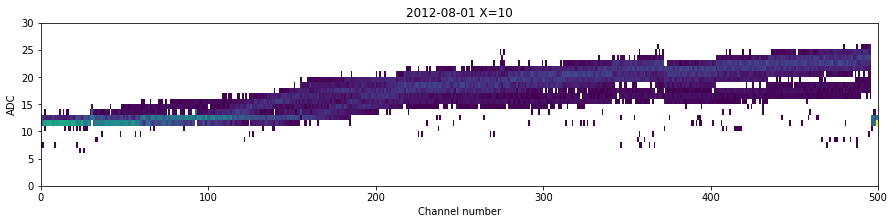
\includegraphics[width=0.7\linewidth]{figures/chapter4/outlierness/real_data.png}
    \caption{}
    \label{plot:real-data}
  \end{subfigure}

\begin{subfigure}[b]{\textwidth}
    \centering
    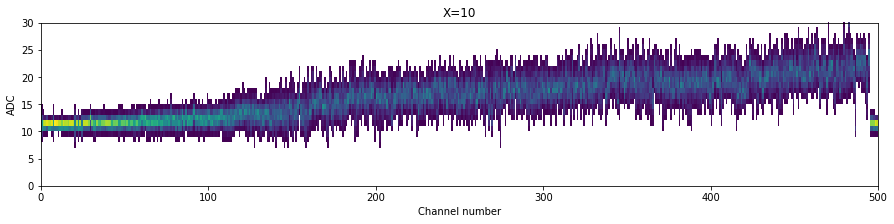
\includegraphics[width=0.7\linewidth]{figures/chapter4/outlierness/generated_data.png}
    \caption{}
    \label{plot:generated-data}
  \end{subfigure}


\begin{subfigure}[b]{\textwidth}
    \centering
    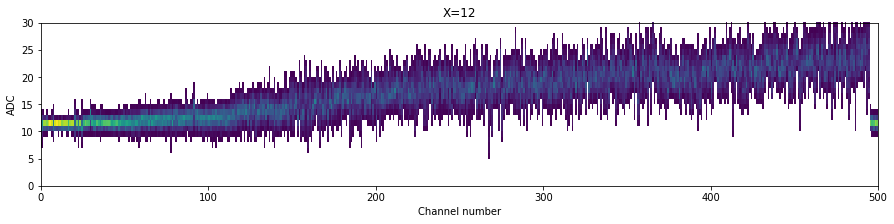
\includegraphics[width=0.7\linewidth]{figures/chapter4/outlierness/generated_x12.png}
    \caption{}
    \label{plot:generated-12}
  \end{subfigure}
    \caption{500 channels from a (a) single calibration date marked with X=10, (b) an example of a single generated calibration parameters at X=12, (c) an example of a single generated calibration parameters at X=12.}
    \label{plot:outlierness_data_example}
\end{figure}

In Fig. \ref{plot:real-data} there is a sample of the data (500 channels) that comes from one of the improper calibrations.
It can be noted that the range of the $H_{t}$ values is on par with those visible in the plot of the generated dataset Fig. \ref{plot:generated-data}.
 Additionally in Fig. \ref{plot:generated-12} there is a plot of calibration with value $X=12$, which was not present in the dataset and is actually outside the scope of the dataset.

This model was introduced to the Lovell VELO monitoring system in the second half of the year 2018, and was used to monitor the calibration data. The Figure \ref{plot:gui} depicts a screenshot from the monitoring system and shows outlierness levels for sensor \# 21. It is noticeable that the value of the outlierness was slightly elevated in 2017, which is attributed to some changes in the cooling system. It is worth noticing that this algorithm was the first Machine Learning based model specifically trained for purpose of supporting the monitoring tasks in the LHCb experiment. 


\begin{figure}
    \centering
    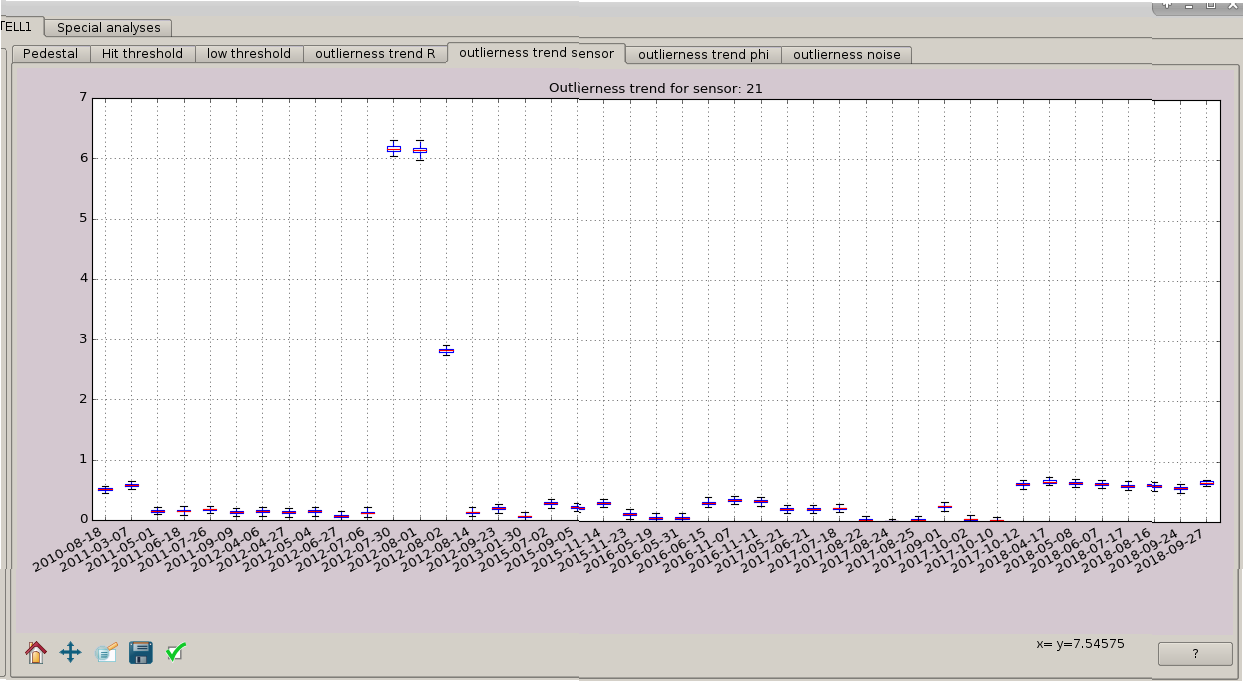
\includegraphics[width=0.7\linewidth]{figures/chapter4/outlierness/calina_lovell_screenshot.png}
    \caption{Screenshot from the outlierness monitoring in Lovell software.}
    \label{plot:gui}
  \end{figure}



  % /////////////////////////////////////////////////////////////////////////
  %
  %
  %
  %
  %                             NEW SECTION
  %
  %
  %
  %
  %
  %





\section{Dimensionality reduction}
\label{chap4:dimred}

The Velo detector, in its strip version, had approximately 172 000 readout channels (that corresponded to physical strips). Many of the parameters needed for its calibration were calculated per channel. This is a huge amount of numbers, which is not easily understandable for human operators.
In its pixel version, the number of such parameters will grow to approximately 41 million (exactly $256*256*12*52 = 40894464$) \cite{Collaboration:1624070}.
Thus, an early test of dimensionality reduction techniques will be very useful for the future. A very popular class of models targeting specifically dimensionality reduction is based on PCA (Principal Component Analysis) or on a particular deep network architecture called the autoencoder.
There are multiple ways of applying PCA or autoencoder to a given dataset (using different sets of values - or dimensions).
This Chapter presents selected applications of dimensionality reduction applied to the VELO calibration dataset.

\subsection{Pedestals dimensionality reduction}

One potential benefit of dimensionality reduction would be to see what differentiates the pedestal parameter in some sensors from the others. For this purpose, we used PCA reduction by reducing each channel's time progression (a single dimensionality reduction for each of the sensor's channels).
This dimensionality reduction can be understood as a mapping:
\begin{align}
  P(n, R, \#, D) \rightarrow X_{n,\#}, X_{n,\#} \in \mathbb{R}^{2}
\end{align}

This means that $X_{n,\#}$ is a 2 dimensional vector, representing an $n$-th channel in $\#$ sensor. 
 Because of the high number of individual sensors, the split into several plots gives more clarity (Fig. \ref{plot:pca_all_peda}, \ref{plot:pca_all_pedb} and \ref{plot:pca_all_ped_phia}, \ref{plot:pca_all_ped_phib}).

  The reduced dataset shows a 2D gaussian distribution.
  It can be seen that some of the channels from a particular sensor can form clusters or be distributed on a ring on the border of the dataset.
  Examining the particular channels can explain what happens with a single datapoint with the transformation.
  In Fig. \ref{plot:PCA_selected} there are three selected channels from a plot of the reduced data in sensor 11.
  Those points are also plotted at the Fig. \ref{plot:PCA_trend}.
  We can see that the channels on the opposing edges of this circle-like structure formed by the reduced data represent different trends in the pedestals' value.
  Channel's 1899 pedestal value grows over time, but 543's decreases.
  Values in channel 322 stay high and stable.
  Therefore we can say that essentially the PCA reduction separates the channels based on their trend.
  The 2-dimensional Gaussian distribution structure makes it consistent with the trend calculation in previous sections, as the distribution centre around 0.
  This means that there is no overall trend (no growth or decrease).
  
\begin{figure}
\centering
  \begin{subfigure}[b]{0.7\textwidth}
    \centering
    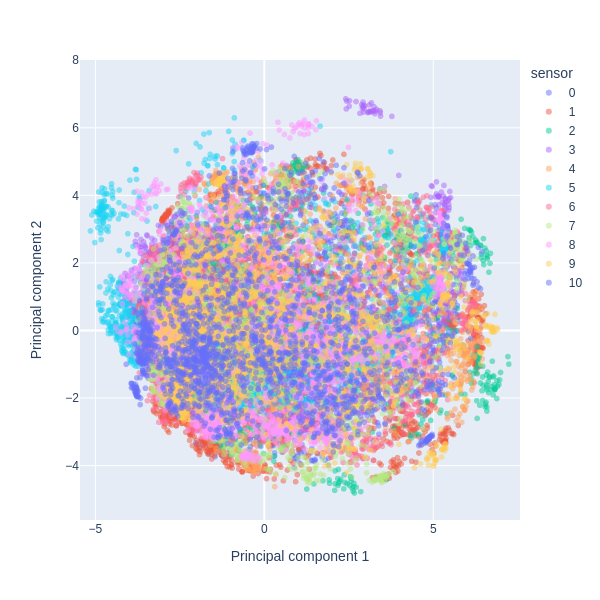
\includegraphics[width=\linewidth]{figures/chapter4/dimred/PCA_pedestals_r_phi_0.png}
    \caption{PCA, $R$-type sensors 0-10}
    \label{plot:PCA_pedestals_0}
  \end{subfigure}
  \begin{subfigure}[b]{0.7\textwidth}
    \centering
    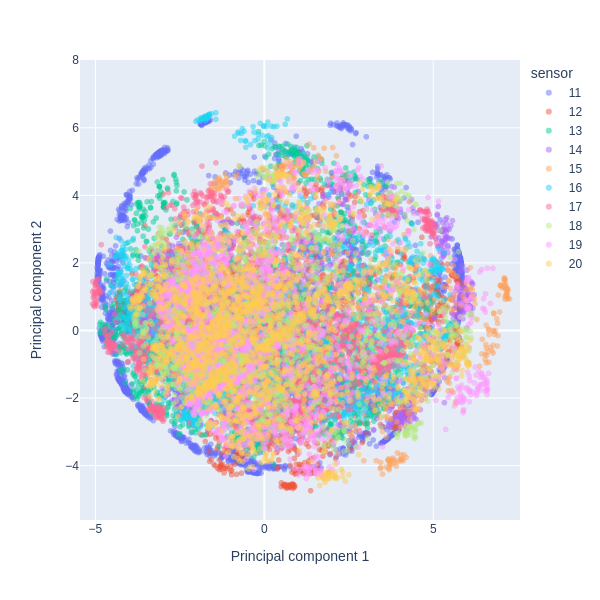
\includegraphics[width=\linewidth]{figures/chapter4/dimred/PCA_pedestals_r_phi_1.png}
    \caption{PCA, $R$-type sensors 11-20}
    \label{plot:PCA_pedestals_1}
  \end{subfigure}


\caption[All calibrationa]{Pedestal calibrations in $R$-type sensors (0-20) reduced with PCA.}
\label{plot:pca_all_peda}
\end{figure}

\begin{figure}
\centering
  \begin{subfigure}[b]{0.7\textwidth}
    \centering
    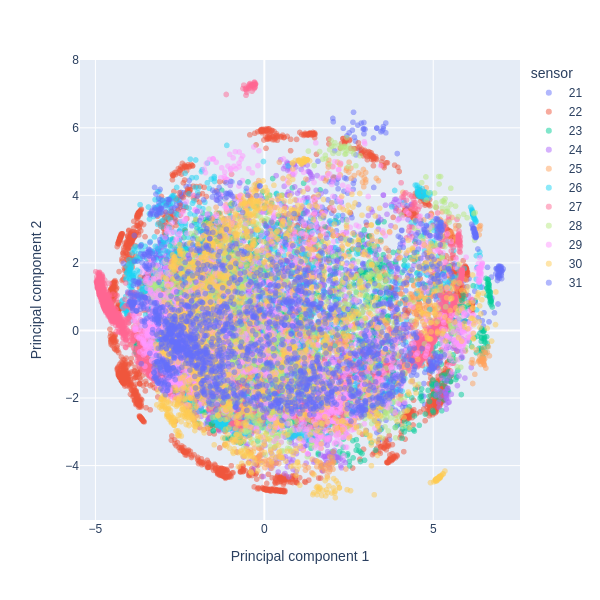
\includegraphics[width=\linewidth]{figures/chapter4/dimred/PCA_pedestals_r_phi_2.png}
    \caption{PCA, $R$-type sensors 21-31}
    \label{plot:PCA_pedestals_2}
  \end{subfigure}
  \begin{subfigure}[b]{0.7\textwidth}
    \centering
    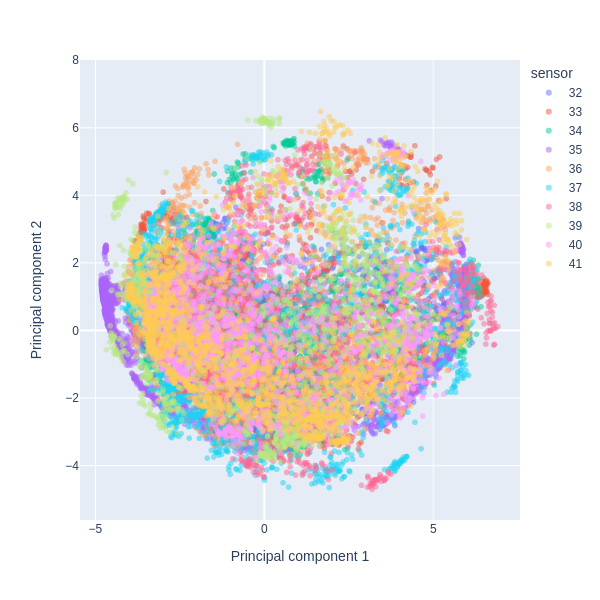
\includegraphics[width=\linewidth]{figures/chapter4/dimred/PCA_pedestals_r_phi_3.png}
    \caption{PCA, $R$-type sensors 32-41}
    \label{plot:PCA_pedestals_3}
  \end{subfigure}

\caption[All calibrationb]{Pedestal calibrations in $R$-type sensors (21-41) reduced with PCA.}
\label{plot:pca_all_ped}
\end{figure}



 \begin{figure}
\centering
\begin{subfigure}[b]{0.7\textwidth}
    \centering
    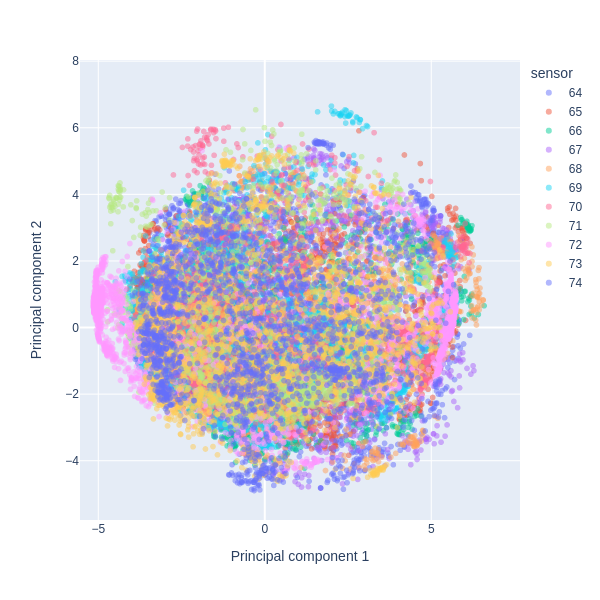
\includegraphics[width=\linewidth]{figures/chapter4/dimred/PCA_pedestals_phi_0.png}
    \caption{PCA, $\Phi$-type sensors 64-74}
  \label{plot:PCA_pedestals_0_phi}
  \end{subfigure}
\begin{subfigure}[b]{0.7\textwidth}
    \centering
    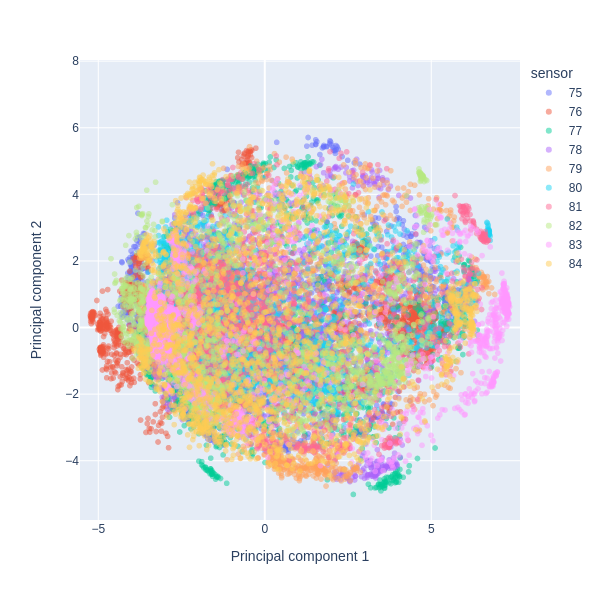
\includegraphics[width=\linewidth]{figures/chapter4/dimred/PCA_pedestals_phi_1.png}
    \caption{PCA, $\Phi$-type sensors 75-84}
   \label{plot:PCA_pedestals_1_phi}
  \end{subfigure}

\caption[All calibrationd]{Pedestal calibrations for $\Phi$-type sensors (64-84) reduced with PCA.}
    \label{plot:pca_all_ped_phia}
\end{figure}

 \begin{figure}
\centering
\begin{subfigure}[b]{0.7\textwidth}
    \centering
    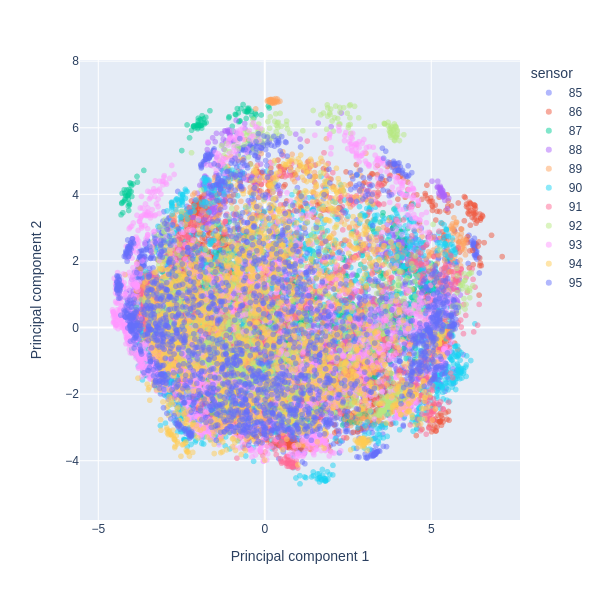
\includegraphics[width=\linewidth]{figures/chapter4/dimred/PCA_pedestals_phi_2.png}
% \caption{}
    \caption{PCA, $\Phi$-type sensors 85-95}
    \label{plot:PCA_pedestals_2_phi}
  \end{subfigure}
\begin{subfigure}[b]{0.7\textwidth}
    \centering
    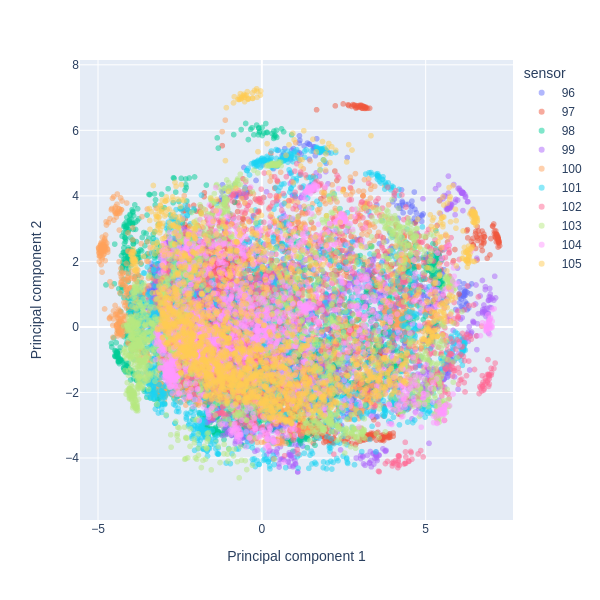
\includegraphics[width=\linewidth]{figures/chapter4/dimred/PCA_pedestals_phi_3.png}
    \caption{PCA, $\Phi$-type sensors 96-105}
% \caption{}
   \label{plot:PCA_pedestals_3_phi}
  \end{subfigure}

\caption[All calibrationd]{Pedestal calibrations for $\Phi$-type sensors (85-105) reduced with PCA.}
    \label{plot:pca_all_ped_phib}
\end{figure}




\begin{figure}[H]
    \centering
    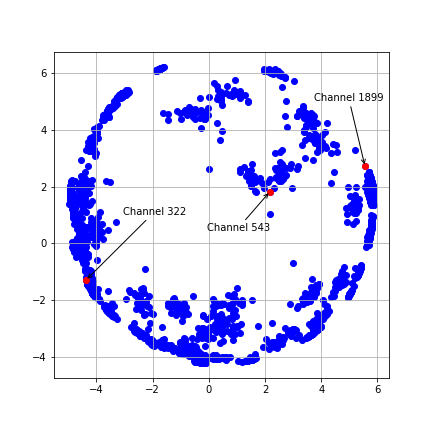
\includegraphics[width=0.5\linewidth]{figures/chapter4/dimred/selected_channels_ped.png}
    \caption{A 2-dimensional representation of the PCA-reduced dataset for sensor 11, with three distinct exemplary channels marked.}
   \label{plot:PCA_selected}
  \end{figure}
  
  \begin{figure}[H]
    \centering
    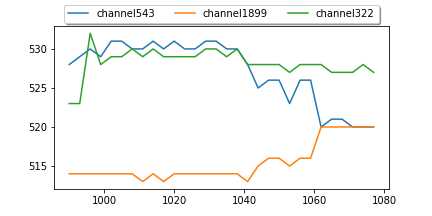
\includegraphics[width=0.6\linewidth]{figures/chapter4/dimred/PCA_trends_channel.png}
    \caption{Time progression of the pedestal value for the selected values.}
   \label{plot:PCA_trend}
  \end{figure}

\subsection{Threshold dimensionality reduction}

Because threshold data for the $R$ and $\Phi$-type sensors differ significantly, it's necessary to split the dimensionality reduction into two cases respectively.
That means training the chosen algorithm for the $H_{t}(Ch*, R, s, d)$ and $H_t(Ch*, \Phi, s, d)$ separately.
This transformation can be written as Eq. \ref{eq:thr_red_R} and \ref{eq:thr_red_phi}.

\begin{align}
  H_{t}(Ch*, R, \#, d) \rightarrow X_{\#,d}, X_{\#,d} \in \mathbb{R}^{2}
  \label{eq:thr_red_R}
\end{align}
\begin{align}
  H_{t}(Ch*, \Phi, \#, d) \rightarrow X_{\#,d}, X_{\#,d} \in \mathbb{R}^{2}
  \label{eq:thr_red_phi}
\end{align}
The two separate models reduce the dimension of the channels into two dimenstions. The $X_{\#,d}$ means that for each sensor $\#$ on given calibration date $d$ there is a dimensional vector $X$.
This form of reduction allows us to easily see any changes common to all of the sensors at once. For studying the high threshold parameters two models, PCA and autoencoder artificial neural network, were used.
In Figures \ref{plot:pca_progression_phi}-\ref{plot:nn_progression_phi} high thresholds for ten consecutive calibrations are plotted after the dimensionality reduction. In this case the high thresholds measured at one sensor with dimensionality $n_{dim}=2048$, corresponding to all physical readout channels, are reduced to a single point on a 2-dimensional ($n_{dim}=2$) plane.
Respective sensors are colour coded for convenience.
Regardless of the used model, PCA or autoencoder, one can clearly see two outlying calibrations 2012-07-30 and 2012-08-01.
In contrast with an autoencoder, the PCA is deterministic and does not require random initialisation. Because of this, there may be some variance in autoencoder model results, even when using exactly the same setup. This may, in some cases, make the PCA based reduction more robust.

\begin{figure}[H]
    \centering
    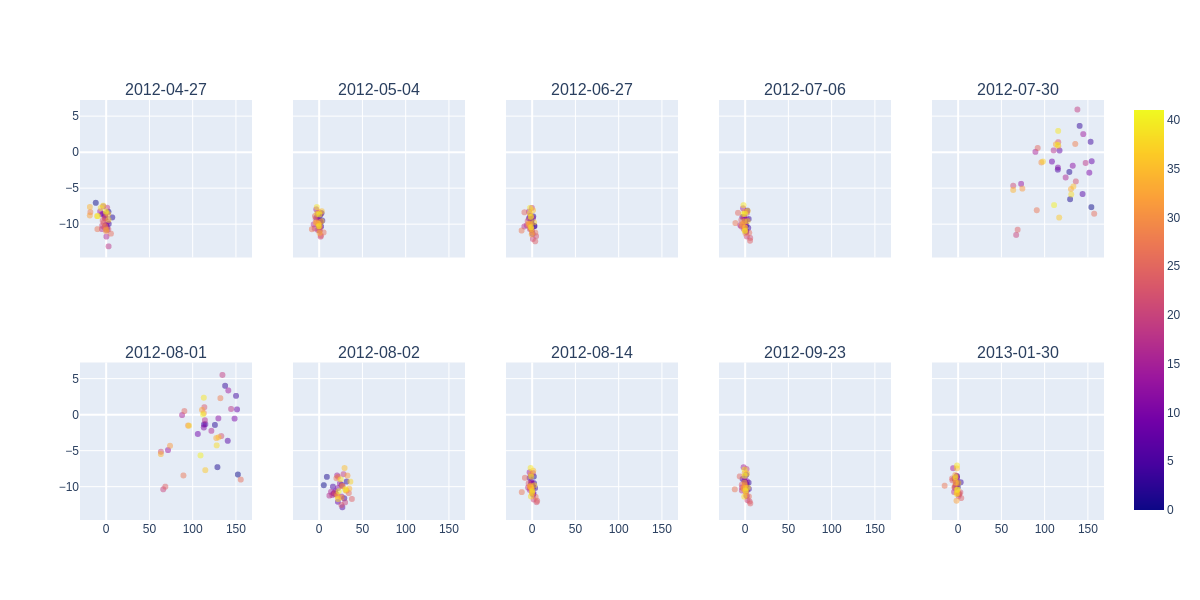
\includegraphics[width=\linewidth]{figures/chapter4/dimred/PCA_module_R_together.png}
    \caption{Time progression of the selected section of calibration dates, with reduced dimentionality using PCA, only for $R$-type sensors.}
   \label{plot:pca_progression_phi}
  \end{figure}

\begin{figure}[H]
    \centering
    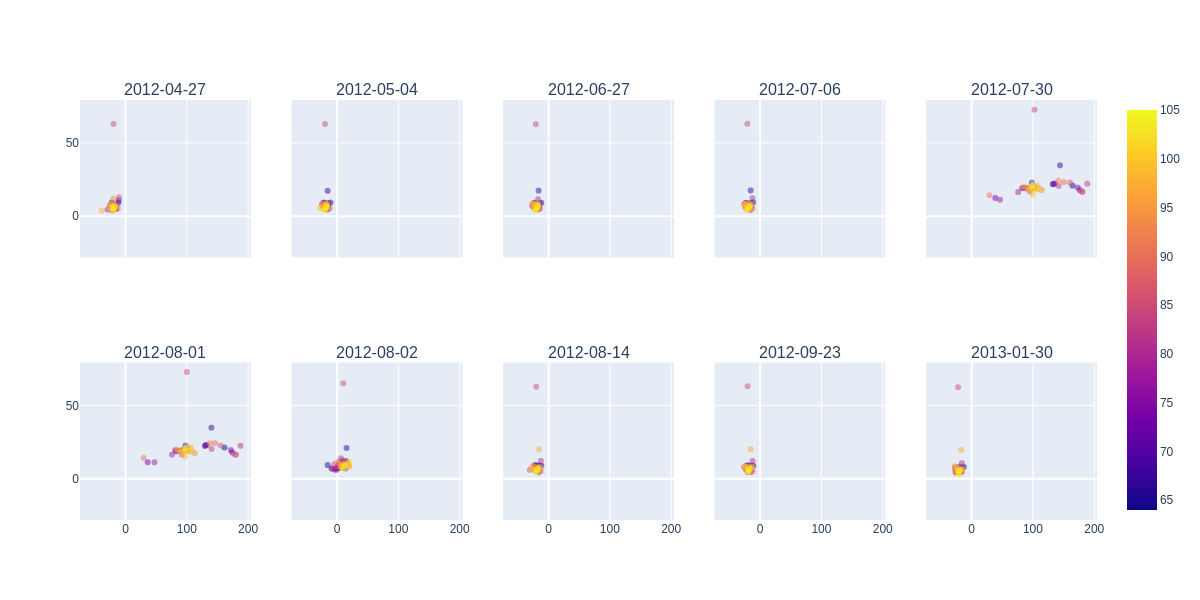
\includegraphics[width=\linewidth]{figures/chapter4/dimred/PCA_module_phi_together.png}
    \caption{Time progression of the selected section of calibration dates, with reduced dimentionality using PCA, only for $\Phi$-type sensors.}
   \label{plot:pca_progression_r}
  \end{figure}

\begin{figure}[H]
    \centering
    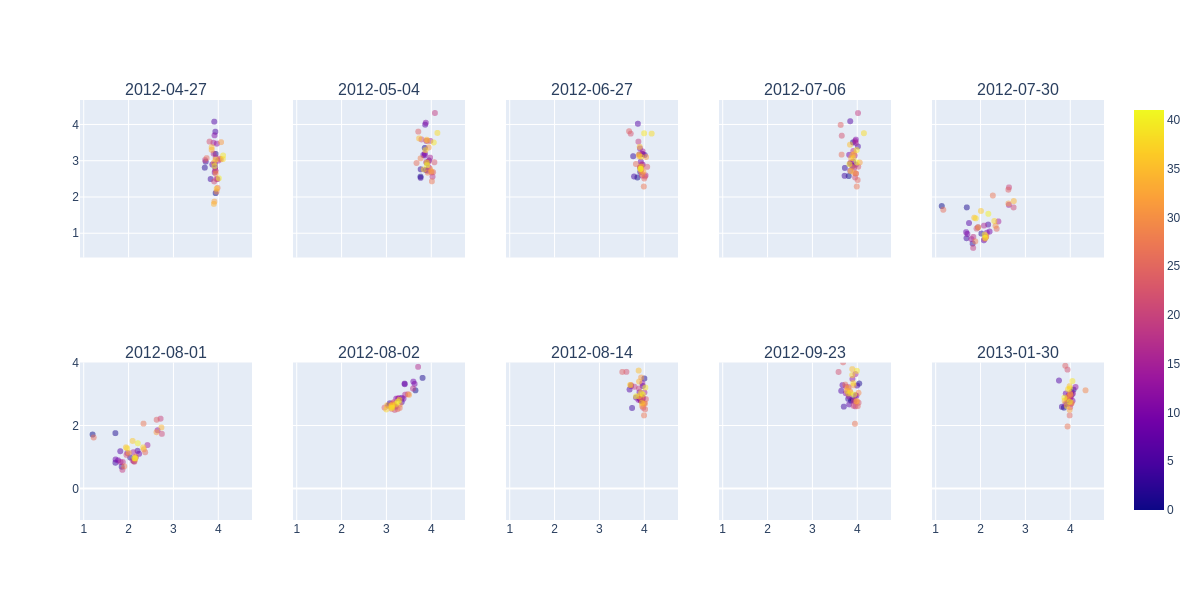
\includegraphics[width=\linewidth]{figures/chapter4/dimred/NN_module_R_together.png}
    \caption{Time progression of the selected section of calibration dates, with reduced dimentionality using an autoencoder, only for $R$-type sensors.}
   \label{plot:nn_progression_r}
  \end{figure}

\begin{figure}[H]
    \centering
    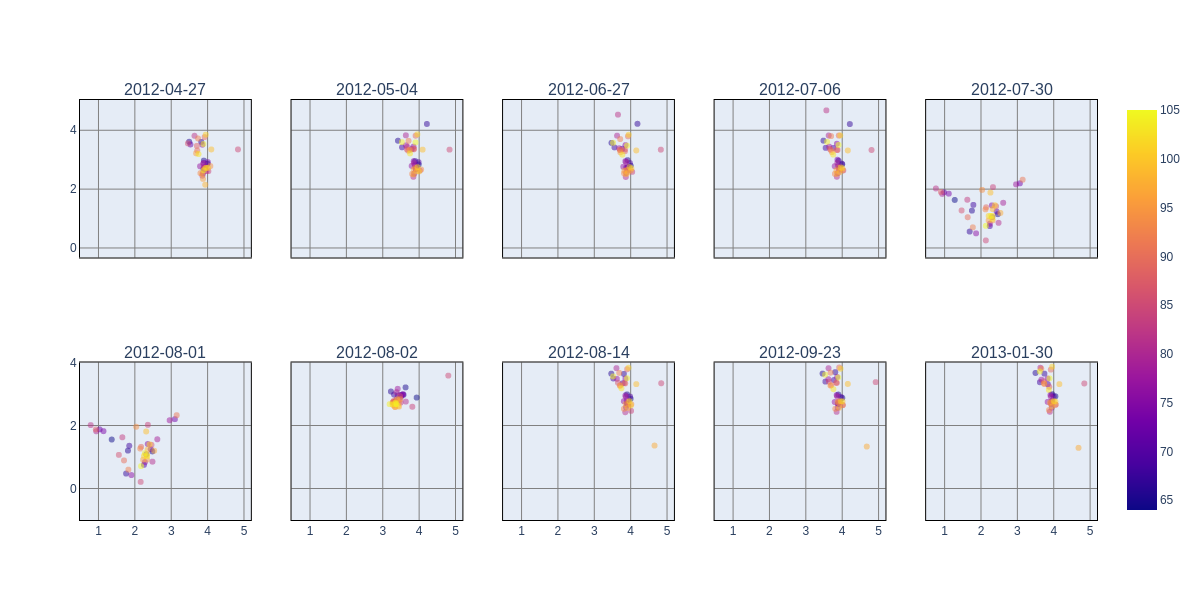
\includegraphics[width=\linewidth]{figures/chapter4/dimred/NN_module_phi_together.png}
    \caption{Time progression of the selected section of calibration dates, with reduced dimentionality using an autoencoder, only for phi sensors.}
   \label{plot:nn_progression_phi}
  \end{figure}

  The Figures \ref{plot:pca_all_r}-\ref{plot:nn_all_phi} represent all calibration dates on the same plot, split into different sensors, and created with different techniques. Notice that all of the plots have different axes scales, as the methods used to reduce dimensionality do not retain the scale. The most helpful insight to those plots is that the relative change represents outlying calibrations.

\begin{figure}
\centering
\begin{subfigure}[b]{0.9\textwidth}
    \centering
    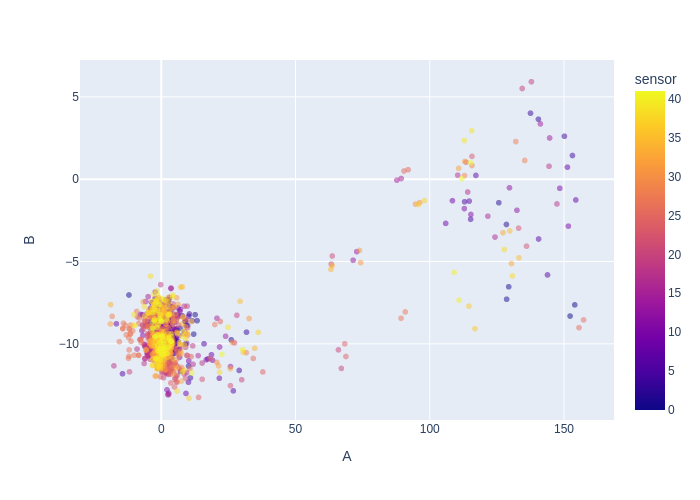
\includegraphics[width=\linewidth]{figures/chapter4/dimred/PCA_module_R_all.png}
\caption{PCA, $R$ sensor type}
   \label{plot:pca_all_r}
  \end{subfigure}
\begin{subfigure}[b]{0.9\textwidth}
    \centering
    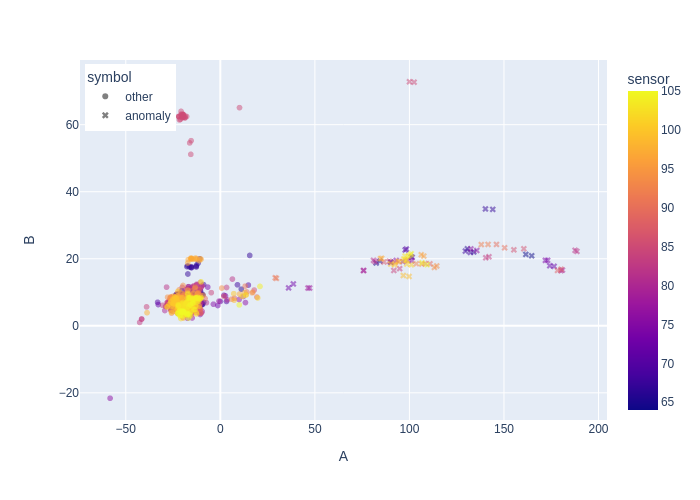
\includegraphics[width=\linewidth]{figures/chapter4/dimred/PCA_module_phi_all.png}
\caption{PCA, $\Phi$ sensor type}
   \label{plot:pca_all_phi}
  \end{subfigure}

    \caption[All calibrationa]{All of the calibrations, with reduced dimentionality using PCA.}
\end{figure}

\begin{figure}
\centering
\begin{subfigure}[b]{0.9\textwidth}
    \centering
    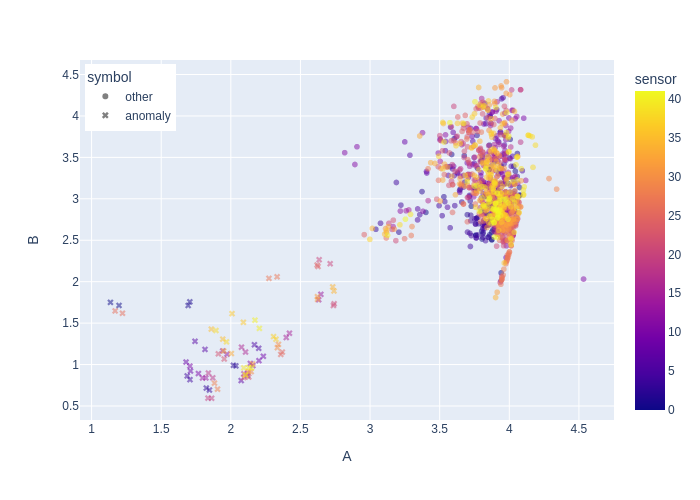
\includegraphics[width=\linewidth]{figures/chapter4/dimred/NN_module_R_all.png}
% \caption{}
\caption{autoencoder, $R$ sensor type}
   \label{plot:nn_all_r}
  \end{subfigure}
\begin{subfigure}[b]{0.9\textwidth}
    \centering
    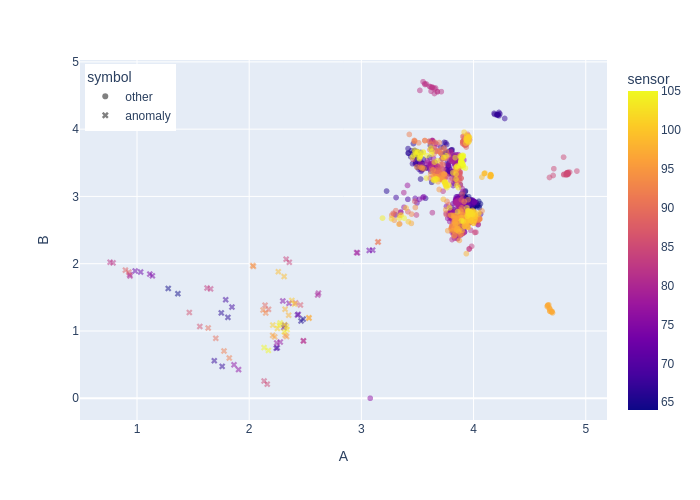
\includegraphics[width=\linewidth]{figures/chapter4/dimred/NN_module_phi_all.png}
\caption{autoencoder, $\Phi$ sensor type}
% \caption{}
   \label{plot:nn_all_phi}
  \end{subfigure}

    \caption[All calibrationd]{All of the calibrations, with reduced dimentionality using autoencoder.}
\end{figure}

  % /////////////////////////////////////////////////////////////////////////
  %
  %
  %
  %
  %                             NEW SECTION
  %
  %
  %
  %
  %
  %
\section{Time to the next calibration forecasting}
\label{chap4:wtte}
%The calibration of the detector is essential for its proper use. It sets the detector's parameters that will be needed during the data taking.
%During LHC Runs 1 and 2, it was possible that if the channel thresholds were set too high, valuable data could be lost. When an electrical signal coming from a single strip would not exceed the threshold, it would be discarded.
%Therefore the detector operations must have as frequent calibrations as possible.
%But the calibration process requires noise data recorded when there is no beam present. Ideally, the longer it takes to register the noise, the better the calibration accuracy (Gaussian noise mean calculation). This also means that calibration requires a particular time slot between data taking when no beam is present.

The calibration procedure requires a special LHCb trigger activity and had to be always planned with great deal of care. This special data taking task was performed during no-beam time slots and due to the complicated Velo system at least one expert must have been present. Also, the RAW data necessary for the calibration are of completely different nature than the regular physical data taken during proton-proton collisions. A typical event size from the entire detector amounted to a few kB during Run 1 and 2, whilst, a single RAW data event from Velo (no suppression, signal is written out from each detector channel) amounted approximately to 190 MB. That large amount of data sent through the trigger system put an enormous stress on it. Also, the significant volume of data challenged each time the disk storage system. Due to its complexity the calibration procedure was run approximately once per month. The data was then processed and the benchmark calibration parameters were evaluated and uploaded to the memory of Tell1 boards. 

All these inconveniences related to the calibration data taking motivated a study on an intelligent method of predicting the necessity of the calibration based on the detector's current condition. The studies performed with the machine leaning approach are described in Section.

\subsection{Dataset}

The calibration data stream contains, in principle, two related types of data: RAW data and setup parameters (also called calibration parameters). The latter are extracted by a set of algorithms, identical for all calibration dates, from the RAW data.
The RAW data contains, in turn, signals registered on each readout channel during no-beam time slot.
%The actual way of calculating the values present in the data does not differ.

%\begin{figure}
 %   \centering
 %   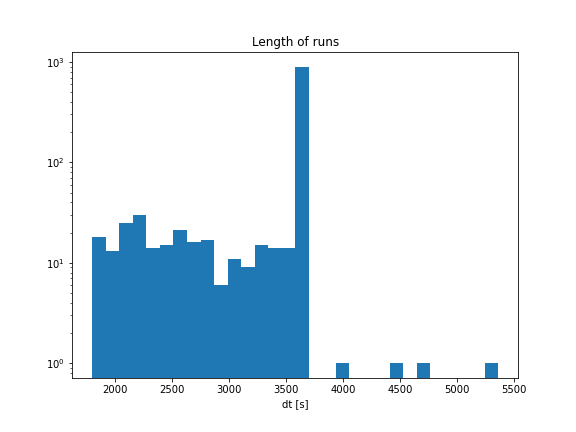
\includegraphics[width=0.6\linewidth]{figures/chapter4/wtte/runlengths.png}
 %   \caption{Histogram of lengths of runs in the dataset expressed in seconds. A significant amount of runs lasted about 3600 seconds (1 hour).}
 %   \label{plot:runlen}
 % \end{figure}
  
%The number of datapoints is significantly more significant for the raw data, as it was taken in any single data run, which can last from a few seconds to about an hour.
%Calibration data, on the other hand, was taken every few weeks.
%In both kinds of the data, there is a constant dimentionality of the parameters, as each of the values was taken for each of the 2048 channels of the sensor individually, giving a 172 032 values of a single parameter for the whole detector.

The statistical analysis of the calibration parameters' trends, described previously, has indicated a candidate for a key quantity that could be used to identify a need for the next calibration. Since, the pedestals turned out to be critical for the quality of the data produced by the vertex detector the analysis focused on them. It was observed, that the pedestal subtracted data slowly drifted, as a function of time, to the point where the data quality was no longer acceptable. During the regular operation a 1-dimensional histogram, also called the summary pedestal histogram, with pedestal subtracted values evaluated on each channel, was used as an observable related to the data quality. Formally, one can define the $\Delta\mu$ as:
\begin{equation}
    \Delta\mu = \mu_{current} - \mu_{calibration}
\end{equation}
Where $\mu_{current}$ is the mean of all pedestal subtracted data coming from the current run and $\mu_{calibration}$ all pedestal subtracted data evaluated after the calibration. Since, the calibration should produce the flat baseline (i.e., the mean value measured at each channel should be centred at 0 ADC), the 1-dimensional summary histogram after the calibration was expected to be approximately normal with the mean value equal to 0 ADC counts and variance close to 0.5 ADC counts. Now, one can analyse the time evolution of the summary histograms produced for RAW data taken at later times\footnote{RAW data samples were also taken during regular physics runs for the monitoring purposes. Usually, for a long run a few thousands of RAW events were taken.} with respect to a given calibration parameters. The main premise being, that the drifting pedestals should affect the summary histogram in a specific way. The study of the $\Delta\mu$ was not conclusive, which is compatible with previous analysis that showed no clear trend in pedestal values over the time.
However, the analysis of the variance, $\sigma(\Delta\mu)$, showed a clear trend in time. An example of this is presented in Fig.
\ref{plot:wtte1-stdevs}. These results show that the width of subsequent summary plots getting larger, thus, $\sigma(\Delta\mu)$ steadily grows in time.

\begin{figure}
\centering
\begin{subfigure}[b]{1.\textwidth}
    \centering
    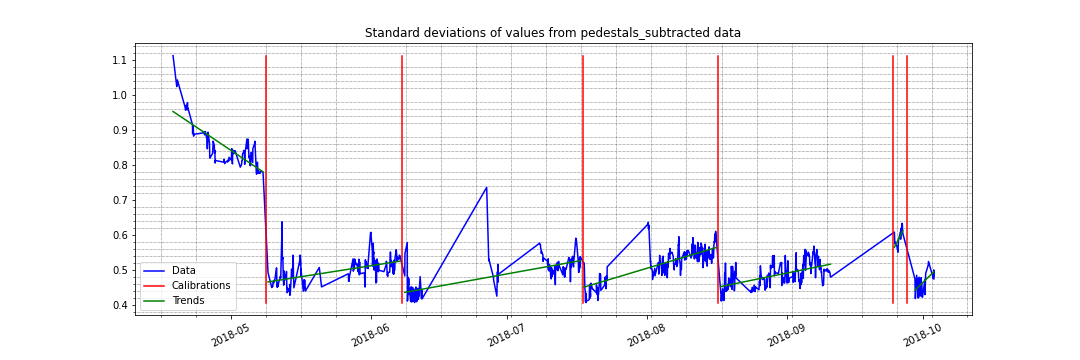
\includegraphics[width=\linewidth]{figures/chapter4/wtte/stdevs_trends_calibs.png}
\caption{}
    \label{plot:wtte1-stdevs}
  \end{subfigure}

\begin{subfigure}[b]{1.\textwidth}
    \centering
    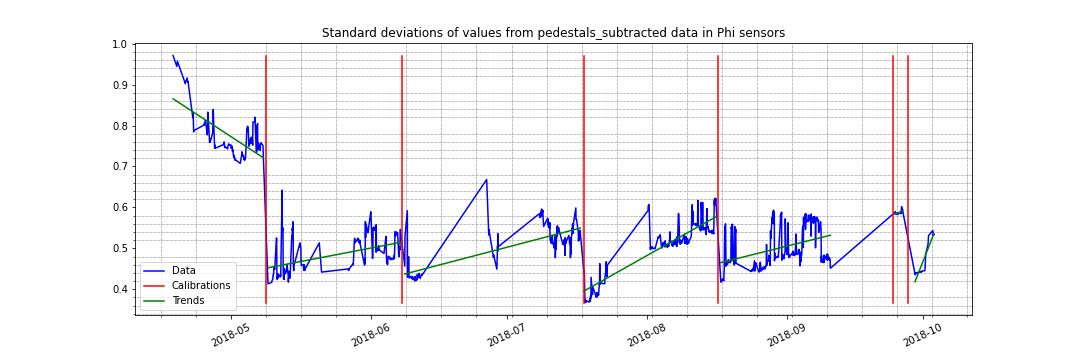
\includegraphics[width=\linewidth]{figures/chapter4/wtte/pstdevs_trends_calibs.png}
\caption{}
    \label{plot:wtte1-p-stdevs}
  \end{subfigure}

\begin{subfigure}[b]{1.\textwidth}
    \centering
    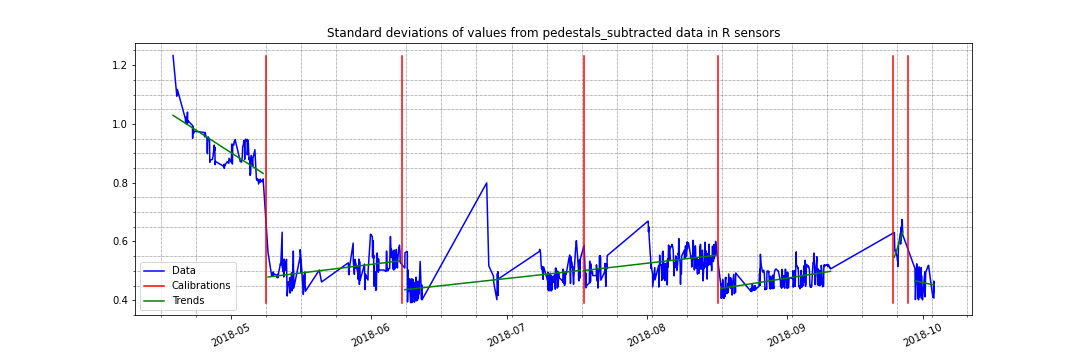
\includegraphics[width=\linewidth]{figures/chapter4/wtte/rstdevs_trends_calibs.png}
\caption{}
    \label{plot:wtte1-r-stdevs}
  \end{subfigure}
  \caption[Two numerical solutions]{$\sigma(\Delta\mu)$ plotted for the whole detector (top), $\Phi$-type sensors (middle), and in $R$-type sensors (bottom). Dates of the benchmark calibrations are marked as red vertical lines for convenience, the green lines correspond to linear trends calculated between calibrations.}
\end{figure}

The data used for the forecasting model comes from 2018. The respective calibration RAW data sets collected in 2018 show the best quality and in this year the calibrations were performed relatively frequently comparing to the previous years (e.g., in 2017 only two calibrations were performed). The more frequent calibrations are related with the radiation damage effects that started to be very pronounced in 2018. The exact time span of the data is from 2018-05-08 to 2018-09-24.
This constitutes exactly four calibration periods. The used data comes in the form of $\sigma(\Delta\mu)_{n}$ where $t$ stands for a given run time.
The time information is translated to delta time ($dt_{n} = t_{n}-t_{n-1}$). 
Both of the vectors are used to craete an input $X_{n}$.

\begin{equation}
X_{n} = \begin{bmatrix} \sigma(\Delta\mu)_{n} \\ dt_{n} \end{bmatrix}
\end{equation}

The continuous-time series of data is transformed to windowed time series of 100 data points, beginning with the first data point after calibration and padded with zeroes.
The padding here means that the the $\sigma(\Delta\mu)$ vector calculated at the first input looks like this: $[0, 0, 0, ..., 0, 0, \sigma_{0}]$ and the next one $[0, 0, 0, ..., 0, \sigma_{0}, \sigma_{1}]$ etc. The analogical padding was used for the $dt_{t}$.

As it is a case of supervised learning, the additional component $Y_{n}$ is set to be a number of days left until the next calibration.
We have chosen the number of days as the most suitable time range for this purpose, as there can be many runs per day.
In practice, it means that the input to the neural network is a vector with 42 values + 1 value for the time difference.
The used model is a version of a recurrent neural network, which means that the temporal dimension of the data can be modulated.
In this case, the model is trained using 100 vectors long sequence.


\subsection{WTTE-RNN model for Velo}

The WTTE-RNN, as discussed in Sec. \ref{sec:wtte_rnn} is capable of outputting the parameters of the Weibull distribution.
The actual type of problem, related to analysis of the time ordered events, in machine learning is called survival analysis. The architecture of the neural network used for forecasting is presented in Table \ref{tab:network}.
It contains six layers in total. The LSTM layer is necessary for the time series, that is used as input data, in order to retain the knowledge on time relation between the analysed events.

\begin{table}[h]
% https://app.neptune.ai/mmajewsk/wtte-calib/e/WTTEC-83/source-code?path=source_code&file=dense_module.py&attribute=files&filePath=.
\begin{center}
\begin{tabular}{ |c|c|c| }
\hline
Layer No. & Layer type & Layer size\\
\hline
1 & Dense & 43\\
2 & Dropout & \\
3 & LSTM & 20\\
4 & Activation - Tanh & \\
5 & Dense & 2\\
6 & WTTE-Activation & \\
\hline
\end{tabular}
\caption{\label{tab:network}The neural network layers used for the WTTE-RNN model}
\end{center}
\end{table}


\subsection{Training and results}

We used Adam optimiser with 400 epochs in the training process, with the Weibull log-like discrete loss. The batch size was equal to 50.


\begin{figure}
\centering
\begin{subfigure}[b]{0.49\textwidth}
\centering
    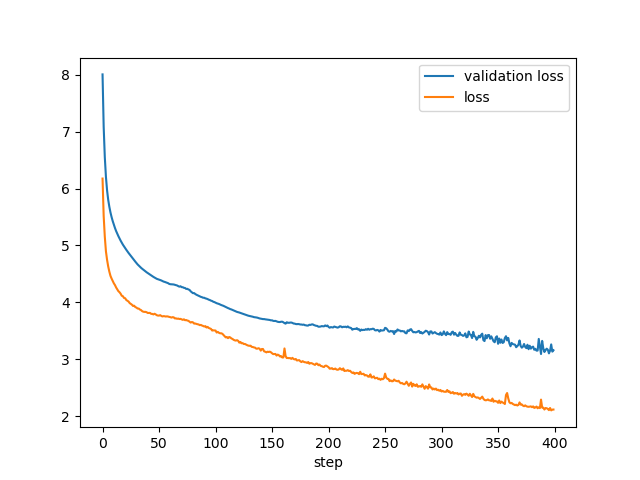
\includegraphics[width=\linewidth]{figures/chapter4/wtte/loss.png}
    \caption{The loss metrics during the training of the WTTE-RNN.}
    \label{plot:wtte_loss}
\end{subfigure}
\begin{subfigure}[b]{0.49\textwidth}
    \centering
    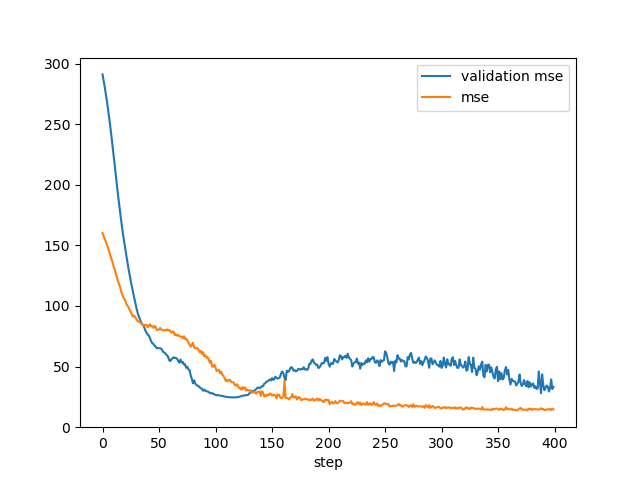
\includegraphics[width=\linewidth]{figures/chapter4/wtte/mse.png}
    \caption{The mean square error metrics during the training of the WTTE-RNN.}
    \label{plot:wtte_mse}
\end{subfigure}
    \caption{The training process of the model.}
    \label{plot:wtte_training}
\end{figure}


The process of the network training is depicted in Fig. \ref{plot:wtte_training}.
You can see that both loss metrics and the additional MSE is decreasing.
For testing purposes, it is helpful to compare the output to the real data.
In Fig. \ref{plot:wtte_realpred} you can see a comparison of the time left to the calibration with the time predicted from our model.
The model is incorrect about its predictions at the beginning, right after calibration, due to a low number of available data points, because the model has less knowledge about current callibration, since it is a new calibration.
It is also visible that the discrepancy between the ground truth and a prediction comes from the large gaps in the subsequent pedestal subtracted data coming from the  in the last weeks of the data taking.
The results shown here are auspicious, but ideally should be confirmed on a larger set of data in the upcoming runs of the LHCb detector.
Because this method relies on the pedestal information, it could be easily adapted to other detectors.

\begin{figure}
    \centering
    \includegraphics[width=\linewidth]{figures/chapter4/wtte/real_vs_predicted.png}
    \caption{Real time to calibration (blue points) and the predicted by the trained WTTE-RNN model (red points)}
    \label{plot:wtte_realpred}
  \end{figure}

\section{Discussion}

This concludes the studies for the strip Velo. 

The analysis in Section \ref{chap4:run12} proves that the Velo maintainers mitigated the radiation damage. The bias voltage introduced to the detector has kept the overall trend of the pedestals close to zero. The noisy channels have been systematically turned off when exhibiting improper behaviours. However, the total number of masked channels was increasing, which is consistent with the expectation of the effect of the ionising radiation.

This analysis also shows that the imperfect calibration process influences the thresholds. We have shown that it can leverage that influence to create a probabilistic programming algorithm for anomaly detection in the calibration.

We have shown that the PCA and autoencoders create a valid candidate for the dimensionality reduction tasks in the space of the calibration parameters for the strip Velo.

The studies of the influence of the calibration on the detector signal have shown that the difference between the calibration pedestal and the mean noise of the signal coming from the channel is growing with time after the calibration and can be used to predict the need for recalibration.

Overall, this research shows promise in the application for the upcoming data taking in Run 3.

  % /////////////////////////////////////////////////////////////////////////
  %
  %
  %
  %
  %                             NEW SECTION
  %
  %
  %
  %
  %
  %

\begin{savequote}[75mm]
Any sufficiently advanced technology is indistinguishable from magic
\qauthor{Arthur C. Clarke}
\end{savequote}
\chapter{Machine Learning methods and analysis for VeloPix}
\label{chap:ml-velo-pix}

While these studies in Chapter \ref{chap:ml-velo} were necessary, they were also the testbed for developing methods that may find use in Run 3 with the upgrade Velo detector.
They also rely heavily on the calibration data recorded during the working of the detector. 
Without the newly upgraded detector working entirely and without the actual data, it is impossible to introduce the same methods before the data taking starts.
Nevertheless, using the test-beam data which was used for finding the optimal configuration of VeloPix ASIC and the experience gained in the process, we can continue research before Run 3.

In the field of particle detectors, one should always be wary of the unexpected. 
The radiation damage or just pure unluck can lead to various scenarios. One of them is a sensor that either introduces too high an amount of variance or behaves unexpectedly.
Similarly to the strip Velo, the VeloPix has mechanisms to silence such a sensor, which renders the detector "blind" in a given sensor.
However, even when the noisy sensors are silenced, another malicious effect still exists, which can harm the reconstruction of the track of particles.
Given an unfortunate grouping (clusters) of the masked pixels in multiple sensors, there can exist a track that the entire detector can be blind to.
This exceptional threat to particle track reconstruction is nearly impossible to be found on a detector calibration with about 65 million individual pixels.
In Section \ref{sec:velopix-mask} we present a novel tool based on an unsupervised learning algorithm for detecting clusters of masked pixels.
We believe this algorithm can be used not only for combatting the particle track reconstruction problem but also broadly for mask cluster tracking in any MediPix family sensor.


The radiation damage in a silicon sensor is a foe most effectively fought off with preparation and awareness.
The Velo detector was designed to be retractable from the collision point. 
This allows for regulation of the amount of particles flowing through the detector, which in another case, could overflow it with data.
However, this also makes a compelling case for measuring the fluence of the detector, as quite literally, it is a moving target.
One would think that since the detector is designed for particle track reconstruction, it would allow for easy calculation of the fluence by counting the hits.
Sadly it is not the case.
The data-taking mode of the VeloPix is focused on selecting the tracks that can be used for physics study purposes and discards all other information.
The rate of the particles incoming to the detector promotes the processing speed and forces not to process more data than is necessary.
The awareness of the radiation damage always comes only after the fact. We cannot measure it before it happens.
Thus, in the VeloPix sensors, there exists a mechanism that is influenced by the damage introduced to the silicon.
By measuring the change in the behaviour of that mechanism, we can determine its damage and, in turn, its fluency.
The surrogate function relates the ToT signal from the sensor to the charge gathered.
The process of calculating the parameters of the surrogate function is de-facto measuring the response of the silicon to the charge deposit. 
This is the mechanism and the link between the fluence and the detector parameters that we can leverage to our advantage.
In the Sec. \ref{sec:surrogates-study} I present the studies of the method for linking the surrogate parameters with the fluence introduced to the sensor.


\section{Intelligent pixel mask cluster tracking}
\label{sec:velopix-mask}
As discussed in Sec. \ref{chap2:velopix_calibration}, the VeloPix masks are essential for filtering signals that otherwise would significantly increase the number of produced noise hits.
In short, the pixels in the VeloPix sensor that exhibit too large noise are ``masked'' - meaning that their readout is deactivated.
The masked pixels are less problematic when they are evenly distributed across the sensor, but when
they cluster together, they can cause a problem for the particle track reconstruction algorithm (Fig. \ref{fig:cluster_masks}).
Simple counting of the masked pixels may not be enough to detect clusters or other structures\footnote{The worst case scenario is a problem with an entire column or row of pixels.} that can be formed by the masked pixels.
%The clustered pixels may be caused by a particle hitting the silicon and causing damage that spills to other pixels.
%This effect, in some cases, may be reversed by annealing the sensors by raising their
%temperature.
%The cluster masks can pose a threat to the reconstruction algorithm and the radial reconstruction resolution.
During a regular operation of a properly configured pixel sensor we expect that the distribution of masked channels should be flat and random and should not feature any accumulation points or structures. Due to its critical impact on the data quality the masking procedure is going to be, arguably, the most important for the daily operation of VeloPix detector. Precise, robust and fast analysis of the masked channels will play a vital role and cannot just include a simple counting algorithm but should also offer more sophisticated metrics. For instance, per sensor analysis of the masked channel density distribution as a function of the channel position. 

\begin{figure}[h]
\centering
\includegraphics[width=0.5\textwidth]{figures/chapter4/velopix_clusters/dbscan_clusters.png}
\caption{An example of clusterisation performed using DBSCAN ($\epsilon$ = 10, MinPts = 4) on the binary pixel-map. Clusters are numbered 1-5.}
\label{fig:dbscan_clusters}
\end{figure}


\begin{figure}[h]
\centering
\includegraphics[width=\textwidth]{figures/chapter4/velopix_clusters/pixel clusters.pdf}
\caption{A visualisation of the problem of the clustered masks. Both images contain a represenataion of multiple aligned sensor matrices pixels, with particle tracks marked with lines. The left image contains uniformly distributed masks, while the right one containse clustered masks. Both cases have the same number of masked pixels.}
\label{fig:cluster_masks}
\end{figure}

\subsection{Simulation of the VeloPix masks}

Due to the VeloPix being still under development and commissioning during these studies the real calibration data  were not available at the time of this analysis. Instead, a dedicated readout system built in the microelectronics lab at AGH-UST was used to produce a fake mask files. Each such file contains 255 x 255 masks that can be uploaded to the memory of VeloPix chip to configure it. The masks can take on two values zeor or one, where zero stands for good channel and one for channel to be masked. The position of the mask is directly mapped to a position of a channel on the sensor.
%the experience gained with the tests of VeloPix was used to create a simulation of occurring masks.
To make a realistic simulation, we have considered the following scenarios:

\begin{itemize}[noitemsep]
  \item Random uniform changes $P$, in which a random portion of pixels changes their state to masked
  \item Linear cluster $L$ where a linear portion of pixels are masked.
  \item Blob cluster $G$ with masks created by a 2D isotropic Gaussian distribution.
\end{itemize}

These scenarios were created to reproduce some effects observed during the preliminary lab tests of the Velo pixel sensors.
These intrusions are added to an initially empty mask file with a different probabilities. Each of the intrusions is created and added to an empty mask matrix to form a single simulated matrix $A$.
One crucial step of this simulation is a random cleaning of the mask matrix, where a random fraction 
%80\% 
of the bad pixels are set back to a no-masked state.
The pseudocode, describing the fake mask files generation, can be found in Listing \ref{alg:two}.
This process creates a continuous simulation of VeloPix mask matrices, as the new masks and clusters are generated and the old ones slowly disappear. In this way we could simulate multiple sensors and multiple calibration runs.

\begin{center}
\begin{algorithm}[H]
\caption{Steps of the mask cluster simulation.}\label{alg:two}
\KwData{$n \geq 0$}
\KwResult{$y = x^n$}
$N \gets n$\;
\While{$N \neq 0$}{
  \uIf{random() $< blob\_prob $ }{
    $A \gets A + G$
  }
  \uElseIf{random() $< line\_prob $ }{
    $A \gets A + L$
  }
    \Else{$A \gets A + P$}
    $A \gets A + Pu$

    $A \gets N - 1$
}
\end{algorithm}
\end{center}
\subsection{Mask clustering}

It was decided to use machine learning approach for searching for potential ordered structures in mask files. Due to the nature of the data an unsupervised technique was chosen based on clusterisation.
There are many clustering algorithms present in the field of machine learning. Although they all come under the term "clustering", there are multiple different goals that various algorithms can achieve. The most common density search clustering algorithms are DBSCAN and OPTICS. The details of these algorithms are described in Section \ref{sec:clustering}.
In the case of application of the clustering algorithm towards analysis of mask files produced during the calibration, the desired algorithm should be able to differntiate points that belong to a cluster from the outliers.
The two algorithms selected for this study fulfill this requirement.
%@TODO mention that clustering in this case does not mean to cluster all of the point on te matrix


\subsection{Mask cluster features}

After finding mask clusters for a given calibration (a one set of mask files), they can be characterised by a set of features.
\begin{enumerate}
\item \textbf{Position}  {$p_k$ = ($\bar{x_k}$, $\bar{y_k}$}), where $\bar{x_k} = \frac{\sum_{i}^{N^k}x_k^i}{N_k},
    \bar{y_k} = \frac{\sum_{i}^{N^k}y_k^i}{N_k}$.
\item \textbf{Size} $s_k$ = \{$n_k$, $d_k$\} where $n_k$ is the number of pixels in a cluster divided by the mean number of the pixels in the given sensor's clusters.
\item \textbf{Shape} $h_k$ = \{$\alpha_k$, $c_k$\}, where $\alpha_k$ is the directional coefficient of the cluster measured by the fit to the line $y^k(x) = \alpha_k*x + b_k$. The $c_k$ is the roundness of the cluster calculated as it's Pearson Coefficient.
\end{enumerate}
With those metrics, we can then define the spacial characteristic vector as $v_k = [s_k; h_k]$. Then we define a cluster as a set of unique features $cluster_k = {p_k, v_k}$.

\subsection{Mask cluster tracking}

This set of unique features, defined in the previous Section, characterises every cluster found for a given calibration.
The $cluster_{k}$ features are then used to identify cluster $k$ from timestep $t_{n}$ as the same in the timestep $t_{n-1}$.
It is performed by calculating a cosine similarity matrix $M$. The $M$ matrix is calculated in the following manner:

\begin{equation}
    M_{i,j} = \Phi_{i,j} * V_{i,j}
\end{equation}

Where $\Phi$ is defined as:
\begin{equation}
    \Phi_{i,j} = \frac{1}{d_{min}}*\max(d_{min} - D_{i,j}, 0)
\end{equation}

and $ D_{i,j} $ is a distance matrix:
 \begin{equation}D_{i,j} = || p_j - p_i ||\end{equation}

The value $d_{min}$ is set to be a limiting factor. If the distance of centroids of the clusters stays the same, the value is 1., but as the distance approaches $d_{min}$, the value approaches 0.
In the tests of the cluster tracking $d_{min}=10$ was used.
The exemplary pairing of the clusters in consecutive simulation steps is visible in the Fig. \ref{fig:fin_clus} with it's similarity matrix calculation in Fig. \ref{fig:sims}.

\begin{figure}[h]
\centering
\includegraphics[width=0.3\textwidth]{figures/chapter4/velopix_clusters/shape.png}
\includegraphics[width=0.3\textwidth]{figures/chapter4/velopix_clusters/distance.png}
\includegraphics[width=0.3\textwidth]{figures/chapter4/velopix_clusters/similarity.png}
\caption{Rows represent clusters on image A in Figure ~\ref{fig:fin_clus}, columns represent clusters on image B in Figure ~\ref{fig:fin_clus}. Values indicate the Spacial Characteristics Similarity Measure \textit{V} (left plot), and Positional Similarity Measure \textit{$\Phi$} (middle plot). The M matrix is the rightmost plot.
}
\label{fig:sims}
\end{figure}

\begin{figure}[H]
\centering
\includegraphics[width=0.7\textwidth]{figures/chapter4/velopix_clusters/paired.png}
\caption{The algorithm chooses clusters labelled with the same integer as the consecutive generations of the same cluster. Clusters labeled as 'new' are clusters on the time step $t_{n}$ that were absent on time step $t_{n-1}$.}
\label{fig:fin_clus}
\end{figure}

 \subsection{Results}


The DBSCAN and OPTICS algorithms were tested on 3000 consecutive simulation steps of a single sensor evolution in time.
The ground truth in the context of clustering of the masks is not something that can be determined in real-world data.
But the simulation, along with the simulation steps, can attribute any generated mask pixel to its source (random uniform, linear, Gaussian blob), thus providing information that can be used as ground truth.
It is assumed, in this analysis, that the generated pixel should be identified as belonging to a cluster after up to 8 timesteps.
The Table \ref{sample-table} presents a confusion matrix calculated using that ground truth information. The OPTICS algorithm has three times as many false positives as the DBSCAN. On the other hand, it has almost twice more true positives.


\begin{table}[H]
  \caption{Confusion matrix values in 3000 consecutive simulation steps.}
  \label{sample-table}
  \centering
  \begin{tabular}{lll}


    \toprule
    Value     & OPTICS     & DBSCAN \\
    \midrule
    True Negative & 7608 & 16207 \\
    False Positive    & 11680 & 3081      \\
    False Negative     & 1156       & 3167  \\
    True Positive &  5665 &   3654   \\
    \midrule
    Accuracy &  0.51 &   0.76   \\
    Precision &  0.33 &   0.54   \\
    \bottomrule

  \end{tabular}
\end{table}

Both algorithms have been tested for the ability to track the consecutive mask cluster's through the steps of the simulation. Fig. \ref{fig:decay} depicts the number of the masks associated with any cluster starting at the timestep of the introduction of said masked pixel. It is visible that The OPTICS algorithm recognises more pixels as belonging to clusters and for an extended amount of time, whereas the DBSCAN very quickly drops its attention to the pixels.

\begin{figure}[H]
\centering
\includegraphics[width=0.48\textwidth]{figures/chapter4/velopix_clusters/optics_decay.png}
\includegraphics[width=0.48\textwidth]{figures/chapter4/velopix_clusters/dbscan_decay.png}
\caption{The fraction of pixels categorised as belonging to any cluster (Y-axis) in the next consecutive calibrations (X-axis), since the cluster introduction to calibration (number of timesteps $n=300$). The number of detected masked pixels slowly decreases with time. The OPTICS algorithm (left plot) recognises the masked pixels of the clusters as belonging to a cluster (not necessarily the same one) for a more extended amount of time. The DBSCAN is more strict in distinguishing the masked pixels that belong to clusters.
}
\label{fig:decay}
\end{figure}

The important test is the influence of the clustering algorithm on the cluster tracking ability. The Fig. \ref{fig:progress} shows a total number of mask clusters in a given simulation timestep, recognised as new or coming from the previous timestep. It is clear that the cluster tracking with OPTICS detects much more clusters as new, and loses more clusters from calibration to calibration, whereas the DBSCAN is finding fewer new clusters, and retains old ones.

\begin{figure}[H]
\centering
\includegraphics[width=0.48\textwidth]{figures/chapter4/velopix_clusters/optics_progress.png}
\includegraphics[width=0.48\textwidth]{figures/chapter4/velopix_clusters/dbscan_progress.png}
\caption{ The number of clusters classified as being "old" - same as in previous calibration (blue colour), and a number of clusters marked as "new" - not being the same clusters as in previous calibration (orange colour). The left plot belongs to OPTICS, and the one on the right to DBSCAN.
}
\label{fig:progress}
\end{figure}

  % /////////////////////////////////////////////////////////////////////////
  %
  %
  %
  %
  %                             NEW SECTION
  %
  %
  %
  %
  %
  %
\section{Studies of the surrogate activation functions measured with the irradiated VeloPix sensors}
\label{sec:surrogates-study}

%The VeloPix sensor is different from the Velo strip in the data taking mode.
%The former is focused on the binary data taking process, and the latter outputs the analogue signal.
%Although the VeloPix can also work in analogue mode, its primary task is to collect and relay the information about the electric charge gathered.
The LHCb vertex locator upgrade led to a major change in sensor technology to provide a much larger channel density and radiation hardness. Both of these features targeted the need to cope with five times higher particle fluence after the upgrade and could only be realised by using silicon planar pixel sensors. The initial design assumed that the new pixel sensors would be read out in analogue mode. However, simulation studies showed that it would lead to an unmanageable high data stream. Thus, a few years into the project, the decision was made to support only the binary readout for the upgrade Velo detector. Still, there is a dedicated data channel, called ECS (Experiment Control System) link, that allows to send out extended digital data at a low rate. This is essential for taking calibration data and understanding the radiation damage effects and measurement of noise. The information about the deposited energy is measured using the TOT\cite{Esposito:2011} (Time-Over-Threshold) technique. So, instead of measuring voltage pulse amplitudes, the readout electronics measure the time window when the voltage pulse is higher than a set analogue threshold (see Fig. \ref{fig:sur_tot}). One should stress that the TOT is, by definition, a digital signal. In order to properly get the proper relation between the TOT counts and the deposited energy, each pixel should be calibrated via measurement of the so-called surrogate or activation function (see Section \ref{surrogate_func}).
With the ECS data link it will still be possible to take the extended data and measure the charge collection efficiency for the irradiated VELO pixel sensors. The technique that will be used for VELO is the measurement of the MPV (Most Probable Value) value of the Landau deposition curves. Such studies have been performed during dedicated test beam campaigns to evaluate if the new pixel sensors will efficiently operate at the end of the Run 4. One idea, that can possibly bring a significant breakthrough for irradiation studies, pertains to fluence estimation based on the properties of the surrogate function and it's relation to the fluence.
This would bring a novel method for measuring the fluence for VeloPix, and possibly for other sensors of MediPix family.
%In this mode, after the energy deposition on the sensor, the time (counter) that it takes for the electric charge to disperse is tracked (see Fig. \ref{fig:sur_tot}).

\begin{figure}[H]
\centering
\includegraphics[width=0.7\textwidth]{figures/chapter4/surrogates/Schematic-of-the-time-over-threshold-working-mode.png}
\caption{A schematic of the TOT working mode.}
\label{fig:sur_tot}
\end{figure}

\subsection{Surrogate function model}
\label{surrogate_func}

The surrogate function is the analytical model that relates the TOT counts to the generated charge, that in turn, is proportional to the deposited energy \cite{Tsopelas:2016cjb}. In essence, the surrogate function is required for the proper energy calibration of each individual pixel. It is predicted that the surrogate curves may change significantly during the operation time of the VELO detector due to severe radiation damage. Understanding and quantifying such changes is a top priority for predicting the detector behaviour after irradiation.
We also show that using the properties of the surrogate functions one can attempt to evaluate the fluence.

The surrogate function can be approximately modelled using the following analitical formula:

% \begin{equation}
%   \label{eq:surrogate}
%   ToT(q) = g \dot q + ToT_{0} - \frac{c}{q-t} + o
%   \end{equation}

\begin{equation}
  \label{eq:surrogate}
  ToT(q) = p_{0} + p_{1} \dot q - \frac{c}{q-t}
  \end{equation}
The formula depends on four parameters: $p_{0},p_{1},c,t$, and is essentially a combination of linear and hyperbolic functions. There is an underlying assumption that $q > 0$.
An exemplary surrogate function is presented in Fig. \ref{fig:surrogate}.
Starting from the lower values, the surrogate function's hyperbolic part is most dominant. Later, the linear component of the function is most dominant as the deposited energy increases.

\begin{figure}[H]
\centering
\includegraphics[width=0.7\textwidth]{figures/chapter4/surrogates/Dependence-of-the-time-over-threshold-signal-measured-by-a-single-Timepix-pixel-on.png}
% possible other plot
% \includegraphics[width=0.7\textwidth]{figures/chapter4/surrogates/surrogate_example.png}
Dependence-of-the-time-over-threshold-signal-measured-by-a-single-Timepix-pixel-on.png
\caption{An exemplary plot of the surrogate function. Source: \cite{Platkevic:2013}.}
\label{fig:surrogate}
\end{figure}

\subsection{Experimental data}

For the source of the data in our studies, we turn to the dataset collected during one of the test beam \cite{Abba_2016} experiments conducted while developing the LHCb Velo upgrade detector.
Particulary, we are interested in the case where the irradiation of the sensor was performed non-uniformly. That is, that within the sensor different areas have different ammount of total fluence.
This allows to link the parameters of the surrogate (which are calculated on per-pixe basis) with different fluence levels.
The test beam  setup used a Timepix3 telescope device \cite{Akiba_2013} that allows for a very precise charged particles tracking with a track pointing resolution, at the centre of the telescope, close to 2 $\mu m$. The device was also able to provide a timestamp for each track with a resolution of 1 $ns$.
%- a range of sensors placed on two sides of the detector under test (DUT).
%Using the range of multiple sensors allows for a very precise measurement of the beam position at the DUT.

\subsection{Cross sensor study}
The test beam data contained multiple different types of sensors with different irradiation schemes.
Unfortunately, in the entire dataset, only one sensor (designated as S8) is suitable for studying the surrogate activation curves in function of particle fluence.
This is due to the irradiation profile of the sensors and available raw data.
Sensor S8 was the only one with a clear, non-uniform profile of the irradiation.
For easier analysis and better statistics, we group the pixels into bins of simmilar level of fluence.
The S8 sensor was the only one that allowed for a binning of the sensor based on the amount of irradiation that the sensors were exposed to. The S8 is a 200 $\mu m$ thick, Hamamatsu n-on-p planar silicon pixel sensor that is virtually identical to the sensors used in the upgrade Velo detector construction. During the test beam experiment it was connected to the Timepix3 readout chip.
%This sensor is Timepix3 W0009\_G08 with 200 μm n-on-p from Hamamatsu.
%With 450 μm inactive edge, 35 μm implant width.
Although other tested sensors featured uniform irradiation profile, nonetheless, we also investigated their activation curves. 
The main strategy of the analysis was to study the properties of the surrogate function model's parameters distributions before and after the irradiation. 
The respective distributions are presented in Figs. \ref{plot:sensor_surrogate_p1}  and \ref{plot:sensor_surrogate_p2}.
The important feature, from the perspective of our analysis, is that for most of the sensors, the distributions of $p0$ and $p1$ parameters shifted to the left after the irradiation. This shift shows that those parameters are sensitive to the fluence.
For the parameters $c$ and $t$ the trend is not as evident.
%, and we will explain it in the further analysis.

\begin{figure}
\centering
\begin{subfigure}[H]{1.\textwidth}
    \centering
    \includegraphics[width=\linewidth]{figures/chapter4/surrogates/p1_S8_histos.png}
% \caption{}
    % \label{plot:wtte1-stdevs}
  \end{subfigure}

\begin{subfigure}[b]{1.\textwidth}
    \centering
    \includegraphics[width=\linewidth]{figures/chapter4/surrogates/p1_S16_histos.png}
% \caption{}
    % \label{plot:wtte1-stdevs}
  \end{subfigure}

\begin{subfigure}[b]{1.\textwidth}
    \centering
    \includegraphics[width=\linewidth]{figures/chapter4/surrogates/p1_S17_histos.png}
% \caption{}
    % \label{plot:wtte1-stdevs}
  \end{subfigure}

\begin{subfigure}[b]{1.\textwidth}
    \centering
    \includegraphics[width=\linewidth]{figures/chapter4/surrogates/p1_S21_histos.png}
% \caption{}
    % \label{plot:wtte1-stdevs}
  \end{subfigure}

\begin{subfigure}[b]{1.\textwidth}
    \centering
    \includegraphics[width=\linewidth]{figures/chapter4/surrogates/p1_S22_histos.png}
% \caption{}
    % \label{plot:wtte1-stdevs}
  \end{subfigure}

  \caption[Surrogate parameters distribution part 1]{Distributions of the surrogate model's parameters measured using sensors S8, S16, S17, S21 and S22. The rows of plots represent respective sensors, each of the columns of the plots represents a parameter of the surrogate model (p0, p1, c, t).  The colour blue (pre) denotes the distribution before irradiation of a given parameter; the orange colour is the distribution after the irradiation of the sensor.}
\label{plot:sensor_surrogate_p1}
\end{figure}

\begin{figure}[H]
\centering

\begin{subfigure}[b]{1.\textwidth}
    \centering
    \includegraphics[width=\linewidth]{figures/chapter4/surrogates/p1_S27_histos.png}
% \caption{}
    % \label{plot:wtte1-stdevs}
  \end{subfigure}

\begin{subfigure}[b]{1.\textwidth}
    \centering
    \includegraphics[width=\linewidth]{figures/chapter4/surrogates/p1_S29_histos.png}
% \caption{}
    % \label{plot:wtte1-stdevs}
  \end{subfigure}

\begin{subfigure}[b]{1.\textwidth}
    \centering
    \includegraphics[width=\linewidth]{figures/chapter4/surrogates/p1_S30_histos.png}
% \caption{}
    % \label{plot:wtte1-stdevs}
  \end{subfigure}

  \caption[Surrogate parameters distribution part2]{Distributions of the surrogate model's parameters measured using sensors S27, S29 and S30. The rows of plots represent respective sensors, each of the columns of the plots represents a parameter of the surrogate model (p0, p1, c, t).  The colour blue (pre) denotes the distribution before irradiation of a given parameter; the orange colour is the distribution after the irradiation of the sensor..}
\label{plot:sensor_surrogate_p2}
\end{figure}


\subsection{The fluence}

As mentioned previously, the sensor S8 was the only one with well-documented non-uniform irradiation profile.
% The irradiation profile is visible in the plot (@TODO) add the actual irradiation plot here.
For the purpose of this studies, we propose an innovative analysis using an adaptive elliptical binning presented in Fig. \ref{fig:binning}.
This binning allows for assigning fluence values per bin and group the pixels with the same fluence. Such approach not only accommodates in a natural way the actual fluence profile but also allows to evaluate various properties of the sensor, expressed as a function of the fluence, with much greater precision and sensitivity.
The measured fluence per bin is as seen in the table \ref{tab:fluence_per_bin}, the innermost bin has the highest fluence level.
This means that we expect that the effects of the radiation will be most visible in the centre of the studied pixel matrix.

\begin{figure}[H]
\centering
\includegraphics[width=0.7\textwidth]{figures/chapter4/surrogates/p2_binning.png}
\caption{A heat-map of the binning used in the analysis of the fluence. The binning starts from 0 at the centre, and the outermost bin is labelled as 7. Each colour represents a different elliptical binning.} 
\label{fig:binning}
\end{figure}

\begin{table}[h]
\begin{center}
\begin{tabular}{ |c|c|c| }
\hline
Bin label & Fluence [$n_{eq}/cm^{2} \dot 1e^{15}$] & No. pixels \\
\hline
  0 & 7.504 & 2153  \\

\hline
  1 & 7.187 & 6406 \\

\hline
  2 & 6.595 & 10718 \\

\hline
  3 & 5.760 & 15040 \\
\hline
  4 & 4.766 & 13715 \\
\hline
  5 & 3.655 & 12228  \\
\hline
  6 & 2.681 & 5141   \\
\hline
  7 & 1.779 & 135\\
\hline
\end{tabular}
\caption{Table of fluence per bin}
\label{tab:fluence_per_bin}
\end{center}
\end{table}

The visible shifts in the surrogate model's parameters $p0$ and $p1$ distributions (with respect to the irradiation) visible across the sensors (Figs. \ref{plot:sensor_surrogate_p1}, \ref{plot:sensor_surrogate_p2}) are complementary to the shift visible in the sensor S8, when comparing the distributions of these parameters per bin, in the Fig. \ref{plot:surr_s8_bins}.
The parameters distributions are depicted as boxplots, per fluence bin, pre- and post-irradiation.
A detailed explanation of the used boxplot is can be seen in Fig. \ref{fig:boxplot}.
One can notice that the $p0$ and $p1$ parameters, measured for the irradiated sensors, exhibit lower values in comparison to the pre-irradiated ones.
%The $p0$ case is the most noticeable, and $p1$, although in total is lower, the trend doesn't keep up with the fluence.
Interestingly, the trends for both investigated parameters are reversed, the $p0$ increases as a function of fluence, whilst, the $p1$ decreases.
%The behaviour of $p1$ could be explained by the initial unequal distribution of this parameter pre-irradiation.
The $c$ parameter exhibits a more significant variance with slightly elevated values.
$T$ parameter also shows large variance, with a visible overall decrease.

\begin{figure}[H]
\centering
\includegraphics[width=0.8\textwidth]{figures/chapter4/surrogates/Boxplot_vs_PDF.png}
\caption{A plot explaining the scope of the boxplot. The top plot represent the boxplot, with median in the middle. The range of the box spans from Quartile 1 to Quartile 3. The interquartile region (IQR) is the width of the box. The whiskers span from the edges of the box to length of 1.5 IQR to either side of the axis.
  The two bottom plots explain the ranges in terms of percentages and width of the distribution. Additionaly, an outlier is a value lying outside the both whiskers range. }
\label{fig:boxplot}
% source: https://towardsdatascience.com/create-and-customize-boxplots-with-pythons-matplotlib-to-get-lots-of-insights-from-your-data-d561c9883643
% source; https://commons.wikimedia.org/wiki/File:Boxplot_vs_PDF.svg
\end{figure}

\begin{figure}[H]
    \centering
\begin{subfigure}[b]{0.95\textwidth}
    \centering
    \includegraphics[width=\linewidth]{figures/chapter4/surrogates/p2_box_plot0.png}
% \caption{}
    % \label{plot:wtte1-stdevs}
  \end{subfigure}
\begin{subfigure}[b]{0.95\textwidth}
    \centering
    \includegraphics[width=\linewidth]{figures/chapter4/surrogates/p2_box_plot1.png}
% \caption{}
    % \label{plot:wtte1-stdevs}
  \end{subfigure}
\begin{subfigure}[b]{0.95\textwidth}
    \centering
    \includegraphics[width=\linewidth]{figures/chapter4/surrogates/p2_box_plot2.png}
% \caption{}
    % \label{plot:wtte1-stdevs}
  \end{subfigure}
\begin{subfigure}[b]{0.95\textwidth}
    \centering
    \includegraphics[width=\linewidth]{figures/chapter4/surrogates/p2_box_plot3.png}
% \caption{}
    % \label{plot:wtte1-stdevs}
  \end{subfigure}
  \caption[Parameters in s8 bins]{Surrogate model's parameters measured for sensor S8 plotted as boxplots for the respective fluence regions. Left-hand side plots represent parameters for non-irradiated sensor, whilst, the right-hand side ones after irradiation. Note, that the highest fluence bin, on the post-irradiation plots, is the far-left one.}
    \label{plot:surr_s8_bins}
\end{figure}

\begin{figure}[H]
    \centering
\begin{subfigure}[b]{0.45\textwidth}
    \centering
    \includegraphics[width=\linewidth]{figures/chapter4/surrogates/p1_S8_corr_pre.png}
% \caption{}
    % \label{plot:wtte1-stdevs}
  \end{subfigure}
\begin{subfigure}[b]{0.45\textwidth}
    \centering
    \includegraphics[width=\linewidth]{figures/chapter4/surrogates/p1_S8_corr_post.png}
% \caption{}
    % \label{plot:wtte1-stdevs}
  \end{subfigure}
  \caption[Corelation surrogate params]{Pearson correlation coefficients between the surrogate parameters in pre- and post-irradiation cases.}
    \label{plot:corr_matrix}
\end{figure}


When analysing the parameters, it is important to note their correlation.
The Pearson correlation parameters presented in Fig. \ref{plot:corr_matrix} show a high correlation between $c$ and $t$ pair, as well as $c$ and $p1$.
We do not explore the reasons for such correlation but acknowledge it in further studies.

\begin{figure}[H]
\centering
\includegraphics[width=1.\textwidth]{figures/chapter4/surrogates/p2_bins_surrogates.png}
\caption{Average surrogate functions plotted for selected fluence regions. Broken lines shows the measured curves before the irradiation, the solid ones after irradiation.}
\label{fig:example_sur}
\end{figure}

To better understand the evolution of the surrogate functions, we present some exemplary activation curves, plotted using the mean value for each respective parameter in selected sensor regions corresponding to appropriate fluence bins.
These exemplary surrogates, plotted for four sensor regions, showed in Fig. \ref{fig:example_sur} are just approximations since we are not de-correlating the parameters, just using the mean values.
In both cases we observe a similar spread of the curves, which is normal, since there is always a spread in physical properties of individual pixels. Interestingly, the spread seems to be approximately the same before and after the irradiation. The most pronounced difference is a significant change in the surrogates' slope after irradiation. This effect can be interpreted as a decrease in charge collection efficiency after irradiation. This is well reflected in the behaviour of the parameter $p1$ - the slope of the activation curve is decreasing as a function of particle fluence. Also, it is visible, alas less clear, that the charge necessary for pixel activation is higher after irradiation. 
%The exemplary surrogates show that for the most part (for more than $1500 e^{-}$ charge), the pre-irradiated sensors expressed more TOT counts for the same amount of charge than after the irradiation.
%Also, although it doesn't have a physical meaning, the plot shows some parts of the surrogates below $0 [TOT]$.
%This is just to show that the surrogate function also changes in other way; the minimum charge required to create a $TOT$ signal is lower.
%But for the majority of the charge range, it means that the sensitivity of the pixels has decreased, which should be expected of the silicon sensors after irradiation.

Given this change in pixels behaviour after irradiation, we can inverse the problem as follows, by measuring the change in the surrogates' parameters before and after the irradiation, it might be possible to estimate the fluence based solely on the data coming from the sensor. One should stress, that this technique may be a major innovation in the field of the silicon radiation studies. So far only unreliable methods of fluence estimations exists based only on Monte-Carlo modelling. Typically, the uncertainty of such modelling is assumed to be at least 100$\%$

\subsection{Modelling the surrogate curves evolution in the fluence domain}

In order to discover the exact nature of the relation of the surrogate parameters with the fluence, we create a statistical model.
As previously shown in Fig. \ref{plot:sensor_surrogate_p1}, the four parameters have a distribution that can be aproximated with a gaussian.
In case of one free parameter this could be done simply by aproximating it's distribution.
With four parameters and partial correlation between them, we need additional steps.
The model, used in our studies, for the surrogates evolution as a function of fluence consists of two parts, rescaling and application of the PCA (Principal Component Analysis). In this way we can generate a large set of surrogate curves that will allow to search for potential pattern of the fluence evolution.
Because the parameters have different ranges of values, scaling is needed to bring them to the same range. We are using a standard scaler in form of ($z = \frac{x - u}{s}$, where $u$ is mean and $s$ is standard deviation ).
Next, because the Pearson coefficient indicates that the parameters are correlated, we will use the PCA to decorrelate them.
%The underlying distributions are not Gaussian, and in fact, the Crystal-Ball distribution would be a better fit.
Since it is easy to decorrelate the variables using the PCA, which assumes that the variables follow the normal (Gaussian) distribution, we will assume Gaussian distribution for the activation curves' parameters.
The PCA internally fits the dimensions of the variables to a 1D Gaussian, and its transformation matrix is holding the width and mean information.
And so the model can be summed in two steps

\begin{enumerate}[noitemsep]
\item Scaling (z= (x-u)/s)
\item Decorrelation with PCA.
\end{enumerate}

The PCA decorrelation allows then for the sampling of the parameters from the decorrelated space using four random Gaussian generators and the following procedure;

\begin{enumerate}[noitemsep]
\item Inverse PCA
\item Inverse scaling (x = (z*s) + u)
\end{enumerate}

This process is useful for checking the loss of the quality of the parameters resulting from assuming that the parameters follow normal distribution.
Fig. \ref{fig:surrogate_model_total} shows the results of applying the model of the surrogates measured for the sensor S8, for all pixels pre-irradiation. It is clear that the generated parameters are of sufficient quality for our purposes (for more detailed studies a more sophisticated model, such as an autoencoder, may be used).
%By separating this model on a per bin basis, we can connect the distribution of the parameter with the fluence.
An additional test for the model is presented in Fig \ref{plot:model_plotted}. The plot depicts the combination of the generated parameters into respective surrogate functions, both using the real world data, and the generated output from our statistical model using learned distribution.

In the two previous tests of the model (Fig. \ref{fig:surrogate_model_total} and \ref{plot:model_plotted}) we were modelling all pixels of the sensor for either pre-irradiated sensor or post-irradiated sensor without the distinction of fluency.
By separating the sensor into 8 distinctive bin areas, we are able to relate the surrogate parameters to the fluence.
For each of the two cases (pre or post-irradiated) and each of the 8 bins, we learn the distribution parameters separately.
The Figs \ref{plot:model_s8_pre} and \ref{plot:model_s8_post} depict the results for the full fluence model, split according to respective sensor regions, are presented. The real-world data and the simulation result are overlayed.
Although we are showing all parameters (p0, p1, c, t), the p0 and p1 have the most substantial impact on the overall shape of the surrogate function.
While in Fig \ref{plot:model_s8_pre} we can see that the distributions in the consecutive bins for the p0 and p1 do not change, in the Fig. \ref{plot:model_s8_post} we can see a noticeable change depending on the bin.
This change corresponds to the change in the fluence in the bins.
What is also important is that in both cases, the real and generated data overlay quite well, showing that our model reflects the change influence.

%instead of crystal-ball.
\begin{sidewaysfigure}
%\begin{figure}[H]
\centering
\includegraphics[width=1.\textwidth]{figures/chapter4/surrogates/p3_model_pipe.png}
\caption{Exemplary results of the surrogate fluence model for the entire sensor. Each column of the plot represents a different parameter of the surrogate function. The first row of plot presents the distribution of respective surrogate model parameters as measured for the sensor S8. The middle row shows the distribution after scaling and applying the PCA, with the Gaussian function fit in orange.
  The bottom row shows the same actual distribution as in the first row in blue, and a distribution of generated parameters using the inverse model procedure.
}
\label{fig:surrogate_model_total}
\end{sidewaysfigure}

\begin{figure}[H]
    \centering
\begin{subfigure}[b]{1.\textwidth}
    \centering
    \includegraphics[width=\linewidth]{figures/chapter4/surrogates/p3_gen_sur.png}
 \caption{Real data}
    % \label{plot:wtte1-stdevs}
  \end{subfigure}
\begin{subfigure}[b]{1.\textwidth}
    \centering
    \includegraphics[width=\linewidth]{figures/chapter4/surrogates/p3_orig_sur.png}
    \caption{Generated data}
  \end{subfigure}
  \caption[has to be capped]{Comparison of true and generated surrogate functions. In case of real data a sample of 300 curves were selected on random from measured data set (plot a). Plot b presents a generated sample of the same size.}
    \label{plot:model_plotted}
\end{figure}


\begin{figure}[H]
    \centering
\begin{subfigure}[b]{\textwidth}
    \centering
    \includegraphics[width=\linewidth]{figures/chapter4/surrogates/p3_histos_pre_0.png}
% \caption{}
    % \label{plot:wtte1-stdevs}
  \end{subfigure}
\begin{subfigure}[b]{\textwidth}
    \centering
    \includegraphics[width=\linewidth]{figures/chapter4/surrogates/p3_histos_pre_1.png}
% \caption{}
    % \label{plot:wtte1-stdevs}
  \end{subfigure}
\begin{subfigure}[b]{\textwidth}
    \centering
    \includegraphics[width=\linewidth]{figures/chapter4/surrogates/p3_histos_pre_2.png}
% \caption{}
    % \label{plot:wtte1-stdevs}
  \end{subfigure}
\begin{subfigure}[b]{\textwidth}
    \centering
    \includegraphics[width=\linewidth]{figures/chapter4/surrogates/p3_histos_pre_3.png}
% \caption{}
    % \label{plot:wtte1-stdevs}
  \end{subfigure}
\begin{subfigure}[b]{\textwidth}
    \centering
    \includegraphics[width=\linewidth]{figures/chapter4/surrogates/p3_histos_pre_4.png}
% \caption{}
    % \label{plot:wtte1-stdevs}
  \end{subfigure}
\begin{subfigure}[b]{\textwidth}
    \centering
    \includegraphics[width=\linewidth]{figures/chapter4/surrogates/p3_histos_pre_5.png}
% \caption{}
    % \label{plot:wtte1-stdevs}
  \end{subfigure}
\begin{subfigure}[b]{\textwidth}
    \centering
    \includegraphics[width=\linewidth]{figures/chapter4/surrogates/p3_histos_pre_6.png}
% \caption{}
    % \label{plot:wtte1-stdevs}
  \end{subfigure}
\begin{subfigure}[b]{\textwidth}
    \centering
    \includegraphics[width=\linewidth]{figures/chapter4/surrogates/p3_histos_pre_7.png}
% \caption{}
    % \label{plot:wtte1-stdevs}
  \end{subfigure}
  \caption[model pre ir]{Comparison of real (blue) and generated (orange) parameters for all fluence regions before the irradiation.}
  \label{plot:model_s8_pre}
\end{figure}

\begin{figure}[H]
    \centering
\begin{subfigure}[b]{\textwidth}
    \centering
    \includegraphics[width=\linewidth]{figures/chapter4/surrogates/p3_histos_post_0.png}
% \caption{}
    % \label{plot:wtte1-stdevs}
  \end{subfigure}
\begin{subfigure}[b]{\textwidth}
    \centering
    \includegraphics[width=\linewidth]{figures/chapter4/surrogates/p3_histos_post_1.png}
% \caption{}
    % \label{plot:wtte1-stdevs}
  \end{subfigure}
\begin{subfigure}[b]{\textwidth}
    \centering
    \includegraphics[width=\linewidth]{figures/chapter4/surrogates/p3_histos_post_2.png}
% \caption{}
    % \label{plot:wtte1-stdevs}
  \end{subfigure}
\begin{subfigure}[b]{\textwidth}
    \centering
    \includegraphics[width=\linewidth]{figures/chapter4/surrogates/p3_histos_post_3.png}
% \caption{}
    % \label{plot:wtte1-stdevs}
  \end{subfigure}
\begin{subfigure}[b]{\textwidth}
    \centering
    \includegraphics[width=\linewidth]{figures/chapter4/surrogates/p3_histos_post_4.png}
% \caption{}
    % \label{plot:wtte1-stdevs}
  \end{subfigure}
\begin{subfigure}[b]{\textwidth}
    \centering
    \includegraphics[width=\linewidth]{figures/chapter4/surrogates/p3_histos_post_5.png}
% \caption{}
    % \label{plot:wtte1-stdevs}
  \end{subfigure}
\begin{subfigure}[b]{\textwidth}
    \centering
    \includegraphics[width=\linewidth]{figures/chapter4/surrogates/p3_histos_post_6.png}
% \caption{}
    % \label{plot:wtte1-stdevs}
  \end{subfigure}
\begin{subfigure}[b]{\textwidth}
    \centering
    \includegraphics[width=\linewidth]{figures/chapter4/surrogates/p3_histos_post_7.png}
% \caption{}
    % \label{plot:wtte1-stdevs}
  \end{subfigure}

  \caption[model post ir]{Comparison of real (blue) and generated (orange) parameters for all fluence regions after the irradiation.}
    \label{plot:model_s8_post}
\end{figure}


\subsection{Particle fluence estimation based on the surrogate curve properties}

Using the model described in the previous Section we can correlate the fluence and the parameters of the surrogate curves. In other words, it should be possible, by analysing the activation curves of an irradiated sensor to recover the fluence level to what the sensor was subjected to. 

Fig. \ref{fig:surrogate_fluence} depicts the most important output of this work. Here we show the exact correlation between the surrogate parameters and the fluence. It depicts the mean and standard deviation of the parameter per fluence bin. In case of $p0$ and $p1$ parameters, there is a clear dependence on the fluence. We can see that the p0 (intercept) is increasing with the fluence, and p1 (slope) is decreasing.
This in accordance with our expectations, as it means that with the same signal (eV) the lower ToT number is produced, which meanse the decrease in sensitivity of the sensor after irradiation.
On the other hand, the dependency of the remaining two parameters $c$ and $t$ is not so clear.
Based on that one can conclude that the fluence has much more impact on the linear part of the surrogate function than on the hyperbolic part.
%of the charge reconstruction is more of an intrinsic parameter tied to the pixel and not strongly correlated to its irradiation.
The hyperbolic part of the surrogate determines the minimum of the generated charge needed to exceed the activation threshold. 
%and threshold calibration is conducted before the data taking.
%Additionally, using the reversal of the fit, it is possible to approximate the fluence that the sensor has experienced.
The progression of the parameter change in respect to fluence is also fitted with a third-degree polynomial, which can be used for inter and extrapolation. This fit can be used for reverse estimation of the fluence based on the surrogate.

\begin{sidewaysfigure}
%%\begin{figure}[H]
\centering
\includegraphics[width=1.\textwidth]{figures/chapter4/surrogates/p3_pre_post_fluences.png}
\caption{Surrogate parameters as a function of particle fluence. These values come from model of the sensor post irradiation. The errorbars denote the standard deviation of the distribution. The blue line is a third degree polynomial fit.}
\label{fig:surrogate_fluence}
%%\end{figure}
\end{sidewaysfigure}

The fluence estimation was cross-checked in the following way. Using the surrogate function evolution model we generated a fake 'irradiated sensor'. These generated activation functions were then used in the simulation software to produce TOT response and reconstruct the Landau deposition functions. The appropriate MPV values taken from the simulated deposites and real ones have been compared in Fig. \ref{plot:landau_example}. As we see the value of measured and simulated MPV agrees very well.
%Using the simulation software, we can try to compare the behaviour of the charge collection distribution for the calibration (surrogates) and the generated surrogates. An exemplary distribution can be visible in the Fig. \ref{plot:landau_example}.
Additionally, we performed the procedure for all fluence bins to get the complete evolution of the MPV value.
The results are presented in Fig. \ref{fig:mpv_vs_fluence}. Again a good agreement between the measured and simulated data is apparent.


\begin{figure}[H]
    \centering
\begin{subfigure}{0.4\textwidth}
    \centering
    \includegraphics[width=\linewidth]{figures/chapter4/surrogates/S8_Elliptic_8Bins_labCalib.png}
    \caption{Ground truth}
    % \label{plot:wtte1-stdevs}
  \end{subfigure}
\begin{subfigure}{0.4\textwidth}
    \centering
    \includegraphics[width=\linewidth]{figures/chapter4/surrogates/S8_Elliptic_8Bins_rndCalib8Bins.png}
    \caption{Generated surrogates}
    % \label{plot:wtte1-stdevs}
  \end{subfigure}
    \caption{Distribution plots of the charge collected in bin 0. The left image shows the distribution made using the actual calibration surrogate functions, and the right image shows the distribution made using generated surrogate functions using our model.}
    \label{plot:landau_example}

\end{figure}

\begin{figure}[H]
\centering
\includegraphics[width=0.9\textwidth]{figures/chapter4/surrogates/mpv_vs_fluence.png}
\caption{The plot of the MPV in different bins, using both the ground truth data and the generated parameters.}
\label{fig:mpv_vs_fluence}
\end{figure}

\section{Disussion}
In this Section, we discussed the purpose of the surrogate function and its meaning in the sensor.
We have shown a correlation between fluence and surrogate parameter values.
We also presented a simple statistical model that describes the surrogate parameter distribution. This model was later used to find the exact nature of the relationship between the surrogates and fluence.
We have shown that this trend can be approximated with a third-degree polynomial.

The results of this work have the following implication: it indicates that it may be possible to use the surrogate calibration to asses the overall fluence experienced by the sensor.
Unfortunately, using only a single sensor and single profile of fluence is not enough to calculate the exact coefficient that would lead to the immediate calculation of the fluence based on the surrogates for the entirety of the VeloPix detector.

However, these methods may be used after the commissioning of the detector by repeating our studies and correlating the surrogates with other means of calculated fluence.

%(@TODO Tomek, please check if I am correct here)
%The studies presented in this section will be beneficial for the future workings of the VeloPix sensors in the LHCb in future runs.
%In comparison with previous mechanisms of measuring the fluence profile for the detector, this method is much faster.
%The disadvantage of this method is that it yet needs confirmation from additional tests that the behaviour exhibited by the S8 is compliant with other sensors.

%%% Local Variables:
%%% mode: latex
%%% TeX-master: "../dissertation"
%%% End:
